\documentclass[11pt,letterpaper]{article}
\usepackage[T1]{fontenc}
\usepackage[utf8]{inputenc}
\usepackage{amsmath,amsthm,mathtools}
\usepackage{newpxtext,newpxmath}
\usepackage[margin=1in,headheight=14pt]{geometry}
\usepackage{microtype}
\usepackage[table]{xcolor}
\usepackage{booktabs,longtable,array}
\usepackage{enumitem}
\usepackage{tikz}
\usetikzlibrary{positioning,arrows.meta}
\usepackage[most]{tcolorbox}
\usepackage{listings}
\usepackage{fancyhdr}
\usepackage{hyperref}
\usepackage[nameinlink,noabbrev]{cleveref}
\definecolor{ink}{RGB}{28,47,68}
\definecolor{teal}{RGB}{18,87,99}
\definecolor{pale}{RGB}{240,246,247}
\definecolor{muted}{RGB}{85,95,103}
\hypersetup{colorlinks=true,linkcolor=teal,citecolor=teal,urlcolor=teal,
  pdftitle={An ordinal Chomp transition at 2},
  pdfsubject={A computer-assisted counterexample to winner stability and to
    the minimal-transition question},
  pdfauthor={Research report prepared for Vladimir Reshetnikov},
  pdfkeywords={Poset games; numerical semigroups; ordinal powers; Apery sets;
    Sprague-Grundy theory; finite-state certificates}}
\pagestyle{fancy}
\fancyhf{}
\fancyhead[L]{\small\color{muted}An ordinal Chomp transition at 2}
\fancyhead[R]{\small\color{muted}Research report}
\fancyfoot[C]{\thepage}
\renewcommand{\headrulewidth}{0.3pt}
\setlength{\parskip}{3.5pt}
\setlength{\parindent}{1.2em}
\setlength{\emergencystretch}{2em}
\setcounter{tocdepth}{2}
\numberwithin{equation}{section}
\newtheorem{theorem}{Theorem}[section]
\newtheorem{proposition}[theorem]{Proposition}
\newtheorem{lemma}[theorem]{Lemma}
\newtheorem{corollary}[theorem]{Corollary}
\theoremstyle{definition}
\newtheorem{definition}[theorem]{Definition}
\newtheorem{example}[theorem]{Example}
\theoremstyle{remark}
\newtheorem{remark}[theorem]{Remark}
\newcommand{\N}{\mathbb N}
\newcommand{\Ord}{\mathrm{Ord}}
\newcommand{\sg}{\operatorname{g}}
\newcommand{\mex}{\operatorname{mex}}
\newcommand{\opt}{\mathcal A}
\newcommand{\Ap}{\operatorname{Ap}}
\newcommand{\Ch}{\mathsf C}
\newcommand{\Norm}{\mathsf T}
\newcommand{\Pout}{\mathcal P}
\newcommand{\Nout}{\mathcal N}
\newcommand{\nimadd}{\mathbin{\oplus_{\!N}}}
\newcommand{\up}{\mathord\uparrow}
\newcommand{\ch}{\operatorname{ch}}
\newcommand{\sat}{\ast}
\newcommand{\smex}{\operatorname{mex}_{\leq 2}}
\newcommand{\pmex}{\operatorname{mex}_{2}}
\newcommand{\R}{\mathcal R}
\newcommand{\J}{\mathcal J}
\newcommand{\HH}{\mathcal H}
\newcommand{\lex}{\mathbin{\mathrm{lex}}}
\lstset{language=Python,basicstyle=\footnotesize\ttfamily,
  keywordstyle=\color{teal}\bfseries,commentstyle=\color{muted},
  stringstyle=\color{teal},showstringspaces=false,columns=fullflexible,
  keepspaces=true,breaklines=true,frame=single,rulecolor=\color{muted!35},
  backgroundcolor=\color{pale!55},framesep=6pt,
  xleftmargin=7pt,xrightmargin=7pt,aboveskip=10pt,belowskip=10pt}
\tcbset{colback=pale,colframe=teal,boxrule=0.6pt,arc=1mm,
  left=10pt,right=10pt,top=8pt,bottom=8pt}

\begin{document}
\begin{titlepage}
\vspace*{0.35in}
{\large\sffamily\color{teal}ORDER THEORY \; / \; ORDINAL COMBINATORICS}\par
\vspace{0.25in}
{\huge\bfseries\color{ink}An ordinal Chomp transition at 2}\par
\vspace{0.15in}
{\Large A computer-assisted counterexample to winner stability\par
and to the minimal-transition question}\par
\vspace{0.35in}
{\large September 20, 2026}\par
\vspace{0.35in}
\begin{abstract}
We refute the winner-stability conjecture for ordinal extensions of
numerical-semigroup Chomp, and we answer negatively the sharper question
asking whether a first-player win must already occur at the first possible
exponent. For each of $S=\langle4,5,6\rangle$ and $S'=\langle4,6,9\rangle$,
Chomp on the semigroup is a second-player win, whereas Chomp on its ordinal
extension below $\omega^2$ is a first-player win. In both cases the least
winning opening, in the usual ordering of ordinals, is $\omega\cdot4+4$,
and the same move wins at every higher exponent. Consequently
$\ch(\{4,5,6\})=\ch(\{4,6,9\})=2$.

The proof isolates a finite spectral statement: every nonempty-parameter
Ap\'ery remainder, with its bottom playable, has Grundy value at least 3.
Equivalently, in the poisoned convention, every such remainder with its
bottom deleted has Grundy value at least 2. We prove this statement by
exact finite-state certificates: nine gap shapes with a seven-row memory
for $\langle4,5,6\rangle$, where the complete state at step 43 repeats at
step 51, and seventeen gap ideals with an eleven-row memory for
$\langle4,6,9\rangle$, where the complete state at step 237 repeats at
step 265. Induction then covers every later parameter. All 387 and 4301
certificate entries are independently checked by direct, untruncated
finite-poset calculations; the 4301 entries for $\langle4,6,9\rangle$ are
checked under both conventions, the 387 for $\langle4,5,6\rangle$ under the
unpoisoned one alone. We give the
order-theoretic reduction, two sufficient criteria for the mechanism, a
general finite-window theorem, two independent descriptions of the winning
responses, both complete certificates, and reproducible Python verifiers
with a regression suite.
\end{abstract}

\vspace{2pt}
\noindent\textbf{Keywords.} Poset games; numerical semigroups; ordinal
powers; Ap\'ery sets; Sprague--Grundy theory; finite-state certificates.
\vfill
\begin{tcolorbox}
\textbf{Status and scope.} This is a computer-assisted research result,
not a peer-reviewed publication or a proof-assistant formalization. It has
not been externally refereed. The finite computations reported here were
executed and cross-checked by separate implementations; ``independently''
means code-level independence, not an external human replication. The
infinite conclusion rests on the proved state recurrence and an exact
state repetition, not on extrapolating a numerical search. No
floating-point arithmetic, random search, external solver, or conjectured
period is involved. Conjecture 4.1 of arXiv:2504.07317v1, dated April 9,
2025, is refuted; Question 4.6 of arXiv:2504.07317v3, dated January 5,
2026, and credited in that revision to Ignacio Garc\'ia-Marco, is answered
negatively. That was the latest source version located. No earlier
resolution was located in the literature search, but that search is not an
exhaustive priority determination, and priority has not been independently
established.
\end{tcolorbox}
\end{titlepage}

\begingroup
\small
\setlength{\parskip}{0pt}
\tableofcontents
\endgroup
\newpage

\section*{Provenance}
\addcontentsline{toc}{section}{Provenance}

This report merges two independently produced research reports on the same
problem. The first, \texttt{ordinal-chomp-transition-at-two}, dated
September 20, 2026 and prepared with ChatGPT in response to a research
request, proves the transition for $\langle4,5,6\rangle$ as its headline
result and carries a second certificate for $\langle4,6,9\rangle$. The
second, \texttt{ordinal-chomp-winner-stability}, dated September 19, 2026
and prepared for Vladimir Reshetnikov, treats $\langle4,6,9\rangle$ alone
and works throughout in the poisoned-board convention. Both dates and both
derivations are recorded here so that the earlier work on the second
semigroup is not silently redated.

The theorem the two reports share, $\ch(\{4,6,9\})=2$ with least winning
opening $\omega4+4$, was proved by the same argument in both: the same
order decomposition, the same three-block detector, and a finite
certificate over the same seventeen gap ideals. A cell-by-cell comparison
confirms that the two certificates record the same 253 rows, agreeing in
all 4301 truncated entries and in all 4301 untruncated values once the
column ordering \cref{eq:column-perm} and the convention shift
\cref{eq:dictionary} are applied. There is one proof here, run on two
semigroups, and it is given once.

Material that genuinely differed between the two sources has been kept
from both and is marked where it appears. The principal such items are the
shift corollary \cref{cor:min-shift}, the free-standing detector
\cref{lem:detector} with \cref{rem:substitution}, the alternative
criterion \cref{prop:criterion}, the block-by-block reply catalogue of
\cref{sec:replies469} beside the invariant argument of
\cref{sec:strategy}, the finite gadget of \cref{sec:gadget}, the complete
$\langle4,6,9\rangle$ certificate table in \cref{app:certificate469}, and
the regression suite described in \cref{sec:checks469}.

\section{The problem and the result}\label{sec:problem}

A numerical semigroup is an additive submonoid $S\subseteq\N$, containing
0, whose complement in $\N$ is finite. Here $\N$ includes 0. Its associated
partial order is
\begin{equation}\label{eq:semigroup-order}
 x\leq_S y \quad\Longleftrightarrow\quad y-x\in S.
\end{equation}
In Chomp, a move deletes the chosen element and all elements above it.
The least element 0 is poisonous: a player forced to take it loses.
Equivalently, remove 0 from the board at the outset and use normal play,
under which a player with no legal move loses.

For an ordinal $\sigma$, form the coefficient extension
\begin{equation}\label{eq:extension}
 S^\sigma=
 \left\{\omega^{\xi_1}s_1+\cdots+\omega^{\xi_k}s_k:
 \sigma>\xi_1>\cdots>\xi_k,\quad s_i\in S\setminus\{0\}\right\}
 \cup\{0\}.
\end{equation}
It carries the order defined by ordinary ordinal subtraction:
$\alpha\leq_{S^\sigma}\beta$ if $\alpha\leq\beta$ and
$\beta-\alpha\in S^\sigma$. The subtraction is characterized by
$\alpha+(\beta-\alpha)=\beta$. In particular, $S^1=S$, while $S^2$ is a
lexicographic product of two copies of the semigroup poset, not their
coordinatewise product.

Rivero Herrera's Question 4.6 asks whether the transition exponent for
these generated ordinal posets is always the smallest possible one
\cite{RH26}; the question is credited in that revision to Ignacio
Garc\'ia-Marco. For finite natural-number generators, that assertion would
mean that whenever some extension is a first-player win, the first
extension already is. The earlier version states the natural-number case
as Conjecture 4.1 \cite{RH25}: it asks whether a second-player win on the
first extension necessarily remains a second-player win on all ordinal
extensions. We call that assertion \emph{winner stability}, and we refute
it. We address precisely the natural-number case; a generic finite-poset
example would not suffice, since the newer paper already distinguishes the
unrestricted poset problem from its algebraically generated
specialization.

Write $\Pout$ for a losing position for the player to move and $\Nout$
for a winning one. For a finite set of positive integer generators
$\Gamma$, define
\[
 \ch(\Gamma)=\min\{\sigma\geq1:\text{Chomp on }
 \langle\Gamma\rangle^\sigma\text{ is }\Nout\},
\]
provided the set is nonempty. We do not assign this minimum when all
extensions are $\Pout$.

\begin{theorem}[Main counterexample]\label{thm:main}
Let $\Gamma=\{4,5,6\}$ and $S=\langle\Gamma\rangle$. Then
\[
 \text{Chomp on }S^\sigma\text{ is }
 \begin{cases}
   \Pout,&\sigma=0,1,\\
   \Nout,&\sigma\geq2.
 \end{cases}
\]
For every $\sigma\geq2$, the least winning first move, in the ordinary
ordinal order, is
\begin{equation}\label{eq:opening}
 \boxed{\omega\cdot4+4.}
\end{equation}
In particular, $\ch(\{4,5,6\})=2$.
\end{theorem}

The answer to the minimal-transition question is therefore negative
already for three small integer generators, and winner stability fails.
No uncountable ordinal, large-cardinal assumption, or change to the game
rules is needed. The same architecture, carried out over a larger gap
poset, gives a second and independent counterexample.

\begin{theorem}[Second counterexample]\label{thm:second}
Let $\Gamma'=\{4,6,9\}$ and $S'=\langle\Gamma'\rangle$.
\begin{enumerate}[label=\textup{(\roman*)},leftmargin=2.2em]
\item Chomp on $S'^{\sigma}$ is $\Pout$ for $\sigma=0$ and $\sigma=1$;
      in particular Chomp on $S'$ itself is a second-player win.
\item Chomp on $S'^{2}$ is $\Nout$. The move $\alpha=\omega\cdot4+4$
      leaves a position of Grundy value 0.
\item The same move wins on $S'^{\sigma}$ for every $\sigma\geq2$, and in
      each such extension it is the least winning first move in the
      ordinary ordinal order. Consequently $\ch(\{4,6,9\})=2$.
\end{enumerate}
\end{theorem}

Part (i) is elementary and uses only the symmetry of this semigroup.
Part (ii) is the substantive calculation: it rests on a finite certificate
for a low-value exclusion, not on a simulation of an infinite board.
Part (iii) holds because the chosen move removes every newly added
higher-order block. \Cref{sec:second} proves all three parts. The second
semigroup is stated here as a theorem in its own right, rather than as a
corollary, because one of the two source reports had it as its headline
result.

\subsection{What is being claimed}

The assertion is a counterexample within the numerical-semigroup family,
not merely within arbitrary pointed partially ordered sets. Winner changes
for arbitrary finite pointed posets are already exhibited in
\cite[Example 3.2]{RH26}, and those examples do not answer the semigroup
question. Conversely, neither counterexample contradicts any asserted
countable upper bound for a transition exponent: each realizes the very
small nontrivial value 2.

The source check for this report found the question still present in the
latest arXiv version, dated January 5, 2026, and found no later
resolution. That is a statement about the literature located in this
investigation, not a claim to have exhaustively searched unpublished work.
The mathematical claim is supported by the complete reduction and the
executable certificates below, independently of its eventual priority
assessment.

\subsection{Proof architecture}

The proof has three logically separate parts. First, an elementary
calculation gives the semigroup's gaps and an Ap\'ery diamond. Second,
Sprague--Grundy algebra turns one excluded option value into a winning
move in the square. Third, a finite-state calculation establishes that
exclusion for every possible first move in the base semigroup.

The infinite conclusion is not obtained by replacing a sufficiently large
finite board by an infinite one. No such approximation is used. The only
limit argument is the induction that follows an exactly repeated state of
a deterministic recurrence.

\subsection{Why the winner changes, and why this problem was tractable}

The outcome of an isolated game records only whether its Grundy value
is zero. A lexicographic substitution can see more: it can depend on
which values occur \emph{one move later}. This suggests looking for a
second-player-winning semigroup whose finite remainders have a small
missing Grundy value. In the examples below, the missing value is 2.
That absence changes the value of a small three-block configuration
from what the individual outcome classes alone would suggest.

In more detail, the poisoned base game loses because all of its first-move
residuals have a maximum. In the square, that maximum becomes an entire
upper copy of the semigroup. Its interaction with two incomparable lower
copies detects a \emph{gap in the option-value spectrum}: the lower pair
has value 0, but its first two excluded option values are 0 and 3, not 0
and 2. Placing a value-1 block above the pair selects the second of these
exclusions, and the independent Ap\'ery diamond contributes another 3, so
the two cancel. The additional ordinal coordinate is therefore not merely
adding more moves to the same strategic situation. It packages the base
game into an ordered compound that can observe more than its winner, or
even than its single Grundy value. That is exactly why a
winner-preservation conjecture can fail.

The decisive calculation is finite but not a bounded experiment. A
numerical semigroup has only finitely many gaps. Those gaps encode all
proper downsets by a moving boundary and finitely many possible tails.
After retaining only the information needed to distinguish values
0, 1, and 2, the boundary evolves by a finite-memory recurrence.
An exact repetition of its entire state proves the desired assertion
for infinitely many Ap\'ery parameters.

\section{Orders, termination, and game conventions}\label{sec:orders}

\subsection{Two games that must not be confused}

For a rooted poset $P$ with least element 0, let $\Ch(P)$ denote its
Chomp game, equivalently the normal-play game on $P\setminus\{0\}$.
Let $\Norm(P)$ denote the normal-play game on \emph{all} of $P$, where
0 is playable and deletes the entire board. Throughout this paper,
$\sg(Q)$ for a finite poset $Q$ means the latter, ordinary normal-play
Grundy value on all listed elements.

This distinction is essential inside a lexicographic product. The
point $(0,0)$ is the only poisoned point. For $a>0$, the bottom
$(a,0)$ of a higher block is an ordinary legal move. Treating every
block bottom as poisoned would produce a different game.

For a finite surviving board $D$ containing 0, we call $D$ itself the
\emph{unpoisoned} board and $D\setminus\{0\}$ its \emph{poisoned}
version. Both occur in the files shipped with this report, and
\cref{sec:dictionary} gives the dictionary between them. Every value
$\sg(\cdot)$ written in this article is the unpoisoned one, so that
$\sg(\Ch(P))=\sg(P\setminus\{0\})$ and $\sg(\Norm(P))=\sg(P)$.

The study of this game, including the symmetric-semigroup second-player
result and the finite-boundary representation used in \cref{sec:window},
originates in Garc\'ia-Marco and Knauer \cite{GMK18}. We prove the
particular facts needed here rather than treating their general theorems
as black boxes.

For a terminating impartial game $G$, put
\begin{equation}\label{eq:sg}
 \opt(G)=\{\sg(G'):G\longrightarrow G'\},\qquad
 \sg(G)=\mex\opt(G).
\end{equation}
The mex is the least excluded ordinal; finite positions have finite
values. A position is $\Pout$ exactly when its value is zero. Infinite
boards in this paper are terminating but need not have a uniform finite
bound on the number of moves. We do not assume finite branching.

\subsection{The lexicographic order at exponent two}

Every member of $S^2$ is uniquely $\omega a+b$ with $a,b\in S$.
If $a<c$, then
\[
 (\omega c+d)-(\omega a+b)=\omega(c-a)+d.
\]
If $a=c$ and $b\leq d$, the difference is $d-b$. It follows that
\begin{equation}\label{eq:lex}
 (a,b)\leq_{S^2}(c,d)
 \quad\Longleftrightarrow\quad
 \bigl(a<_S c\bigr)\ \text{or}\
 \bigl(a=c\text{ and }b\leq_S d\bigr).
\end{equation}
Here $a<_S c$ means $c-a\in S\setminus\{0\}$. Thus unequal comparable
first coordinates make \emph{every} element of the lower block lie
below \emph{every} element of the upper block.

The algebraic construction from natural sums and products of integer
generators gives exactly \cref{eq:extension}: each Cantor coefficient
is an ordinary nonnegative integer combination of the generators.
The order, however, uses ordinary ordinal subtraction, not coefficientwise
subtraction under the natural sum. Our convention \cref{eq:lex} explicitly
supplies the reflexive case and uses a strict comparison of unequal first
coordinates. This also explains why the winning opening must be written
$\omega\cdot4+4$ and not $4\cdot\omega+4$: those are different ordinals,
and only the first is a member of $S^2$.

\subsection{Why no infinite play occurs}

Let $F$ be the largest gap of a numerical semigroup $S\ne\N$. If
$x<y$ and $y-x>F$, then $x<_S y$. Therefore an antichain in $S$ is
bounded in an interval of length $F$, and it is finite. A descending
chain for $\leq_S$ is also a descending chain of natural numbers.
Hence $S$ is a well partial order.

A lexicographic product of two well partial orders with least elements
is again a well partial order. Indeed, the distinct first coordinates
of an antichain must themselves be an antichain, and a fixed fiber
contains only a finite antichain. A descending sequence is excluded
by first stabilizing the first coordinate and then the second, or,
in our ordinal realization, simply by the ordinary ordinal order.

The same reasoning proves by transfinite induction that every
$S^\sigma$ is a well partial order. At a limit stage, two nonzero
ordinals with different leading exponents are comparable: their
highest differing coordinate compares 0 with a positive member of
$S$. An antichain therefore has a fixed leading exponent and belongs
to a smaller successor stage, where the induction hypothesis applies.
The point 0 creates no exception.

In any Chomp play, the chosen sequence $x_0,x_1,\ldots$ satisfies
$x_i\not\leq x_j$ for $i<j$, because an earlier move would otherwise
have deleted the later one. The well-partial-order property excludes
such an infinite sequence. This justifies the terminating-game
recursions used below.

For the two semigroups treated here, a reader can also check termination
by hand, without the general theory. Every play of either game on $S$
terminates because its first move either empties the board or leaves a
finite Ap\'ery set. After the prescribed move in the square only finitely
many blocks remain, and once a block is touched it becomes finite. Hence
all the Grundy values used in the main argument are well defined, even
though some of the games involved have infinitely many options.

\section{The small amount of game algebra needed}\label{sec:algebra}

\subsection{Disjoint and ordinal sums}

The disjoint sum $G+H$ lets a player move in one component and leave
the other unchanged. Its value is
\begin{equation}\label{eq:disjoint}
 \sg(G+H)=\sg(G)\nimadd\sg(H).
\end{equation}
For finite values, $\nimadd$ is bitwise exclusive-or, not Hessenberg
natural sum. The normal-play theorem and the ordinal-sum formula
below are standard; a convenient treatment is
\cite[Sections 2 and 4, especially Theorem 2.6]{GT21}.
We include the part of the proof that controls the counterexample.

The ordinal sum $G:H$ has $G$ below $H$. A move in $H$ preserves $G$;
a move in $G$ discards all of $H$. Therefore its options are $G'$ and
$G:H'$. If $A$ is a set of ordinals, define its excluded-ordinal
enumeration recursively by
\begin{equation}\label{eq:excluded}
 E_A(\eta)=\mex\bigl(A\cup\{E_A(\xi):\xi<\eta\}\bigr).
\end{equation}
It lists the complement of $A$ in increasing order, beginning with
index 0.

\begin{lemma}[Ordinal-sum formula]\label{lem:colon}
For terminating impartial games,
\[
 \sg(G:H)=E_{\opt(G)}\bigl(\sg(H)\bigr).
\]
In particular, if $\sg(H)=0$, then $\sg(G:H)=\sg(G)$.
\end{lemma}
\begin{proof}
Fix $G$ and argue by induction on the game tree of $H$. Moves in $G$
have values in $A=\opt(G)$; by induction moves in $H$ have values
$E_A(\sg(H'))$. Put $\eta=\sg(H)$. No option of $H$ has value
$\eta$, while every $\xi<\eta$ occurs as an option value. Thus
$E_A(\eta)$ is absent from the option values of $G:H$. Every ordinal
below it is either in $A$, or equals $E_A(\xi)$ for some
$\xi<\eta$, and is present. Taking mex proves the formula. The last
assertion is $E_A(0)=\mex A$.
\end{proof}

A first, elementary consequence records what a playable minimum does. It
is quoted repeatedly below, and it is what makes the poisoned and
unpoisoned conventions interchangeable.

\begin{corollary}[Adding a legal minimum]\label{cor:min-shift}
If $D$ is a finite poset with least element 0, then
\begin{equation}\label{eq:min-shift}
 \sg(D)=1+\sg\bigl(D\setminus\{0\}\bigr).
\end{equation}
\end{corollary}
\begin{proof}
Write $D=\mathbf1:(D\setminus\{0\})$, where $\mathbf1$ is the one-point
game: playing 0 in $D$ deletes everything, and every other move leaves 0
in place below the remainder. Since $\opt(\mathbf1)=\{0\}$, the $n$-th
ordinal excluded from $\opt(\mathbf1)$ is $n+1$ for finite $n$. Now apply
\cref{lem:colon}.
\end{proof}

The option spectrum of a disjoint sum also has a simple description:
\begin{equation}\label{eq:option-sum}
 \opt(G+H)=
 \{a\nimadd\sg(H):a\in\opt(G)\}
 \cup\{\sg(G)\nimadd b:b\in\opt(H)\}.
\end{equation}
This follows immediately by considering which component was changed.

\subsection{A low-value detector}

The whole mechanism of this paper is concentrated in the following
lemma, which mentions no posets at all. Isolating it separates the nimber
content from the order geometry, and both criteria below cite it.

\begin{lemma}[The low-value detector]\label{lem:detector}
Let $G$ be a terminating impartial game with $\sg(G)=1$, all values in
$B=\opt(G)$ finite, and
\begin{equation}\label{eq:low-spectrum}
 B\cap\{0,1,2,3\}=\{0,3\}.
\end{equation}
Then
\begin{equation}\label{eq:detector}
 \sg\bigl((G+G):G\bigr)=3.
\end{equation}
\end{lemma}
\begin{proof}
Put $U=G+G$. Then $\sg(U)=1\nimadd1=0$, and by \cref{eq:option-sum},
\[
 C:=\opt(U)=\{b\nimadd1:b\in B\}.
\]
Exclusive-or with 1 exchanges 0 with 1 and 2 with 3, so
\cref{eq:low-spectrum} gives
\[
 1,2\in C,\qquad 0,3\notin C.
\]
These four assertions correspond respectively to $0,3\in B$ and
$1,2\notin B$; option values at least 4 cannot affect them. Hence the
first two ordinals excluded from $C$ are $E_C(0)=0$ and $E_C(1)=3$.
Since $\sg(G)=1$, \cref{lem:colon} gives
$\sg\bigl((G+G):G\bigr)=E_C(1)=3$.
\end{proof}

\begin{remark}[Why a single nimber is not enough]\label{rem:substitution}
Replacing \emph{every} occurrence of $G$ by a singleton would be wrong.
A singleton $\mathbf1$ also has Grundy value 1, yet
\[
 \sg\bigl((\mathbf1+\mathbf1):\mathbf1\bigr)=2,
\]
not 3: here $\opt(\mathbf1+\mathbf1)=\{1\}$, whose first two excluded
values are 0 and 2. The lower components of an ordinal sum therefore
contribute their option \emph{spectrum}, not merely its mex, while the
upper component may be summarized by its Grundy value. The distinction is
systematic in the ordered-join substitution theory of
\cite[Section 4]{GT21}.
\end{remark}

\subsection{A four-point-remainder criterion}

Let $P$ be a rooted well partial order. Abbreviate $C=\Ch(P)$ and
$T=\Norm(P)$. A finite diamond $D$ is the four-element poset with
bottom, two incomparable middle elements, and top. All its points
are playable, and $\sg(D)=3$: deleting the bottom, a middle point,
or the top gives values 0, 2, or 1, respectively.

\begin{proposition}[Spectral mechanism]\label{prop:mechanism}
Suppose $a\in P\setminus\{0\}$ satisfies the following conditions.
The remainder $P\setminus\up a$ is a diamond
$\{0,p,q,r\}$, and $a$ is incomparable with $p,q,r$. Moreover,
\begin{equation}\label{eq:spectral-hypothesis}
 \sg(C)=0,\qquad
 \opt(T)\cap\{0,1,2,3\}=\{0,3\}.
\end{equation}
Then $(a,a)$ is a winning opening in Chomp on $P\lex P$.
\end{proposition}
\begin{proof}
Since $T$ is a playable singleton below $C$, \cref{lem:colon} gives
$\sg(T)=1$. The hypothesis \cref{eq:spectral-hypothesis} is exactly
\cref{eq:low-spectrum} for $G=T$, and all option values of $T$ are finite
because every option is a finite poset. Therefore \cref{lem:detector}
applies and
\begin{equation}\label{eq:V-three}
 \sg\bigl((T+T):T\bigr)=3.
\end{equation}
Explicitly, with $U=T+T$ and $A=\opt(T)$ we have $\sg(U)=0$ and
\begin{equation}\label{eq:U-low}
 \opt(U)\cap\{0,1,2,3\}=\{1,2\},
\end{equation}
whose first two excluded ordinals are 0 and 3.

After the move $(a,a)$, the first-coordinate blocks indexed by
$0,p,q,r$ remain complete, and the block indexed by $a$ becomes
$D=P\setminus\up a$. All other blocks disappear. The poisoned
point lies only in block 0, so that block contributes $C$.
The three blocks at $p,q,r$ contribute $(T+T):T$, while the block
at $a$ is incomparable with all three. The remaining game is exactly
\begin{equation}\label{eq:remaining-general}
 C:\left(D+\bigl((T+T):T\bigr)\right).
\end{equation}
The game in parentheses has value $3\nimadd3=0$. Its ordinal sum
above $C$ therefore has value $\sg(C)=0$. The opening leaves a
$\Pout$-position and wins.
\end{proof}

The condition excluding 2 from the option spectrum is genuinely used.
Knowing only $\sg(T)=1$ excludes 1, but does not determine whether
2 occurs. If 2 occurred, the second excluded value of $\opt(T+T)$
would no longer be forced to equal 3. This is the information lost
by an argument based only on the outcome of an individual block.
\Cref{rem:substitution} makes the complementary point with an explicit
counter-computation.

\subsection{An alternative criterion, with weaker hypotheses}

The second of the two source reports isolated a variant of
\cref{prop:mechanism} that assumes less. We keep both. The version below
buys two things: incomparability is \emph{derived} from atomicity rather
than assumed, and the low-spectrum hypothesis shrinks to the single
exclusion of the value 2, because $0\in\opt(G)$ now comes from the
minimum move and $3\in\opt(G)$ from the diamond option.

\begin{proposition}[Diamond-atom criterion]\label{prop:criterion}
Let $P$ be a pointed poset whose normal and poisoned games terminate, and
write $G=\Norm(P)$. Suppose that
\begin{enumerate}[label=\textup{(\alph*)},leftmargin=2.2em]
\item $\sg(P\setminus\{0\})=0$ and $\sg(G)=1$;
\item $P$ has an atom $a$ for which $P\setminus\up a$ is the four-point
      diamond;
\item $2\notin\opt(G)$, and all values in $\opt(G)$ are finite.
\end{enumerate}
Then $(a,a)$ is a winning first move in Chomp on $P\lex P$.
\end{proposition}
\begin{proof}
The minimum move gives $0\in\opt(G)$; the value $\sg(G)=1$ excludes 1
from $\opt(G)$; the option at $a$ is the diamond, of value 3, so
$3\in\opt(G)$. With (c) this is \cref{eq:low-spectrum} for $G$. The atom
$a$ is incomparable with every positive point of $P\setminus\up a$, since
it is neither above a positive predecessor, being an atom, nor below a
surviving point, by the definition of $\up a$. The residual decomposition
after $(a,a)$ is therefore exactly \cref{eq:remaining-general}, and
\cref{lem:detector} finishes the computation as in
\cref{prop:mechanism}.
\end{proof}

The hypotheses of \cref{prop:criterion} are strictly weaker than those of
\cref{prop:mechanism} in the situations used here, and imply them: given
(a), (b) and (c), the incomparability required by \cref{prop:mechanism}
follows from atomicity, and
$\opt(T)\cap\{0,1,2,3\}=\{0,3\}$ follows as in the proof just given.
The converse does not hold, since \cref{prop:mechanism} does not require
$a$ to be an atom. We nevertheless retain \cref{prop:mechanism} because
it is the form applied verbatim in \cref{sec:semigroup}, where the
incomparabilities are checked directly from the gap list and no atom
argument is needed.

\section{The semigroup \texorpdfstring{$\langle4,5,6\rangle$}{<4,5,6>}}
\label{sec:semigroup}

\subsection{Symmetry and the losing first level}

Let $S=\langle4,5,6\rangle$. The four consecutive integers
$8,9,10,11$ lie in $S$, and adding 4 proves that every integer at
least 8 lies in $S$. Direct inspection below 8 gives
\begin{equation}\label{eq:gaps456}
 S=\N\setminus\{1,2,3,7\},\qquad F=7.
\end{equation}
For $0\leq n\leq7$, exactly one of $n$ and $7-n$ belongs to $S$.
Thus $S$ is symmetric.

For $b\in S\setminus\{0\}$, define the Ap\'ery remainder
\begin{equation}\label{eq:apery}
 R_b=\Ap(S,b)=S\setminus(b+S).
\end{equation}
It is exactly the board remaining after the move $b$ in $S$, before
removing the poisoned 0. It is finite: an element larger than $b+F$
cannot remain. We also set $R_0=\Ap(S,0)=\varnothing$ when using normal
play, which is the value of the move at 0 in $\Norm(S)$.

\begin{lemma}[The symmetric-semigroup argument]\label{lem:symmetric}
Every $R_b$ for $b>0$ has greatest element $b+7$. Consequently
$\Ch(S)$ is a $\Pout$-position.
\end{lemma}
\begin{proof}
The element $b+7$ belongs to $S$ and its difference from $b$ is the
gap 7, so it belongs to $R_b$. If $x\in R_b$ and $x<b$, then
$b+7-x>7$ belongs to $S$. If $x\geq b$, then $x-b$ is a gap,
and symmetry gives $7-(x-b)\in S$. In both cases $x\leq_S b+7$.

A finite normal-play poset $Q$ with a greatest element $m$ is
$\Nout$. To see this, delete $m$. If the result is $\Pout$, that
was a winning move. If not, it has a winning move $z$; playing $z$
in the original poset deletes $m$ as well and gives the same
$\Pout$-remainder. Apply this to $Q=R_b\setminus\{0\}$, which
still has the nonzero greatest element $b+7$. Every legal first
move in $\Ch(S)$ thus leaves an $\Nout$-position, proving the claim.
\end{proof}

This reproduces, in the present small case, the symmetric-semigroup
result of Garc\'ia-Marco and Knauer \cite[Theorem 2.4]{GMK18}.
The extra fact we need is stronger than that outcome statement.

Write $C=\Ch(S)$ and $T=\Norm(S)$. Since $R_b$ for $b>0$ is a finite
poset with least element 0, \cref{cor:min-shift} gives
\begin{equation}\label{eq:root-shift}
 \sg(R_b)=1+\sg\bigl(R_b\setminus\{0\}\bigr).
\end{equation}
In particular, the preceding lemma excludes value 1 for $R_b$.
Also
\begin{equation}\label{eq:spectrum-T}
 \sg(C)=0,\qquad\sg(T)=1,\qquad
 \opt(T)=\{0\}\cup\{\sg(R_b):b\in S\setminus\{0\}\}.
\end{equation}

\subsection{The diamond and the remaining spectral assertion}

A direct calculation gives
\begin{equation}\label{eq:diamond456}
 R_4=\{0,5,6,11\}.
\end{equation}
Its middle points are incomparable because $6-5=1\notin S$;
its top dominates them because $11-5=6$ and $11-6=5$ are in $S$.
Thus it is a diamond $D$, and $\sg(D)=3$.
Moreover, 4 is incomparable with 5, 6, and 11: their differences
from 4 are the gaps 1, 2, and 7.

\begin{lemma}[Certified spectral gap]\label{lem:gap}
For every $b\in\langle4,5,6\rangle\setminus\{0\}$,
\begin{equation}\label{eq:gap}
 \sg(R_b)\geq3.
\end{equation}
\end{lemma}

The proof occupies \cref{sec:window,sec:certificate}. Given this lemma,
\cref{eq:spectrum-T} has low spectrum exactly $\{0,3\}$, and
\cref{prop:mechanism} applies with $a=4$, $p=5$, $q=6$, $r=11$.
The block decomposition after $\omega4+4$ is displayed below.

\begin{figure}[htbp]
\centering
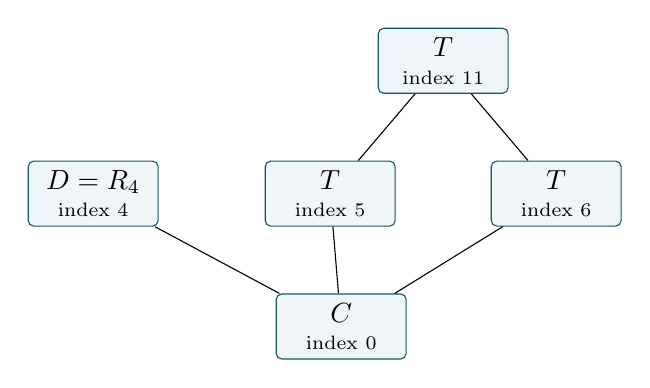
\begin{tikzpicture}[x=1.4cm,y=1.25cm,
  box/.style={draw=teal,rounded corners=2pt,fill=pale,
     minimum width=1.65cm,minimum height=0.68cm,align=center},
  every edge/.style={draw=ink,line width=0.6pt}]
\node[box] (base) at (0,0) {$C$\\[-2pt]\scriptsize index 0};
\node[box] (d) at (-2.25,1.35) {$D=R_4$\\[-2pt]\scriptsize index 4};
\node[box] (p) at (-0.1,1.35) {$T$\\[-2pt]\scriptsize index 5};
\node[box] (q) at (1.95,1.35) {$T$\\[-2pt]\scriptsize index 6};
\node[box] (r) at (0.925,2.7) {$T$\\[-2pt]\scriptsize index 11};
\draw (base)--(d);\draw (base)--(p);\draw (base)--(q);
\draw (p)--(r);\draw (q)--(r);
\end{tikzpicture}
\caption{The remaining blocks, with lower boxes below upper boxes.
Only the global point $(0,0)$ was poisoned. The block at index 4
is detached from the three blocks at indices 5, 6, and 11.}
\label{fig:blocks}
\end{figure}

\subsection{The exact transition and the least winning opening}

The move $\omega4+4$ leaves the game
\[
 C:\left(D+\bigl((T+T):T\bigr)\right)
\]
and hence is winning, once \cref{lem:gap} has been established.
No positive \emph{finite} opening is winning: such a move deletes
every ordinal with a positive higher coefficient and leaves just
$R_b\setminus\{0\}$, which is $\Nout$ by \cref{lem:symmetric}.

The only remaining legal opening below $\omega4+4$ is $\omega4$.
After it, the block at index 4 is absent. The opponent can play
$\omega11$, deleting the top block and leaving
\[
 C:(T+T),
\]
which is $\Pout$, since $\sg(C)=0$ and $\sg(T+T)=0$.
Thus $\omega4$ is not a winning first move either.
There are no intermediate legal coefficients 1, 2, or 3.
This proves minimality of \cref{eq:opening}.

Finally, in $S^\sigma$ with $\sigma>2$, every point whose leading
exponent is at least 2 lies above $\omega4+4$: subtracting the latter
leaves that point itself. The opening therefore deletes every such
point and leaves exactly the same board as it does in $S^2$.
This proves all assertions of \cref{thm:main}, conditional only on
the certified spectral lemma proved next.

\section{A finite-window theorem for low Grundy values}\label{sec:window}

We now give a general reduction, rather than postulating periodicity
for one numerical sequence. Let $S\ne\N$ be an arbitrary numerical
semigroup, $\HH=\N\setminus S$ its gap set, and $F=\max\HH$.
The moving-boundary encoding of downsets follows the locality idea
used in \cite[Section 6]{GMK18}; retaining several low Grundy values
instead of just the outcome gives the recurrence developed here.
No claim of independent priority is made for this general method.

\subsection{Encoding all proper downsets}

Give $\HH$ the order induced by semigroup differences, and let
$\J$ be the finite set of its downsets. For $x>F$ and $C\in\J$, set
\begin{equation}\label{eq:Pxc}
 P(x,C)=(S\cap[0,x))\cup(x+C).
\end{equation}
All these positions include a \emph{playable} 0.

\begin{lemma}\label{lem:tails}
The finite downsets of $S$ whose least missing integer of $S$ is
$x>F$ are exactly the positions $P(x,C)$ with $C\in\J$.
In particular, $R_x=P(x,\HH)$ for $x>F$.
\end{lemma}
\begin{proof}
If $P$ is such a downset and $z\in P$ with $z\geq x$, the difference
$z-x$ cannot belong to $S$, or the missing point $x$ would lie below
$z$. Thus $z=x+g$ for a gap $g$. If $g$ is included and $g-h\in S$
for another gap $h$, then $x+h\leq_S x+g$, so $h$ is included too.
The selected gaps form $C\in\J$.

Conversely, let $C$ be a downset of the gap order. Suppose
$z\leq_S x+g$ with $g\in C$. If $z<x$, it is in the prescribed
prefix. If $z\geq x$, write $z=x+h$. The number $h$ cannot lie
in $S$, because $g-h\in S$ would then imply $g\in S$. Hence
$h\in\HH$, and the downset property puts $h$ in $C$.
This proves that $P(x,C)$ is a downset. Its least missing member
is $x$, since 0 is not a gap. The last assertion follows directly
from the definition of $R_x$.
\end{proof}

This description \emph{refines} the finite-gap encoding of
\cite[Section 6]{GMK18}: beyond the conductor, the admissible tails are
exactly the gap ideals, not arbitrary subsets of the gap set. That is what
makes the number of columns finite and small, seventeen rather than
sixty-four in the larger example below.

\subsection{Truncation without approximation}

Fix $K\geq0$. Define
\[
 \tau_K(n)=\begin{cases}n,&0\leq n\leq K,\\
                          \sat,&n>K.
             \end{cases}
\]
For a set of these symbols, $\mex_{\leq K}$ returns its least absent
member of $\{0,\ldots,K\}$, or $\sat$ if every one is present.
The symbol $\sat$ is not a nimber. Then
\begin{equation}\label{eq:exact-truncation}
 \tau_K\bigl(\mex B\bigr)=
 \mex_{\leq K}\{\tau_K(b):b\in B\}
\end{equation}
for every finite set of option values $B$. Indeed, deciding whether
the mex is a specified number at most $K$ requires knowing only
which option values up to $K$ occur. Therefore computing the
truncated values recursively is \emph{exact}, not a numerical
approximation to larger values.

Put
\[
 v_x(C)=\tau_K(\sg(P(x,C))).
\]
The proof uses $K=2$, but the general statement will be useful for
understanding why a finite certificate is possible.

\subsection{Every move is either far, near, or in the tail}

For a tail move at $x+c$, $c\in C$, the new tail is
\begin{equation}\label{eq:cut}
 C_c=\{g\in C:g-c\notin S\}.
\end{equation}
Negative integers are understood not to belong to $S$. In particular,
$c\notin C_c$, so this is a proper smaller tail.

For a prefix move at $y=x-d$, where $1\leq d\leq F$ and
$x>2F$, define
\begin{equation}\label{eq:delta}
 \Delta_d(C)=\{g\in\HH:g<d\text{ or }g-d\in C\}.
\end{equation}
The new position is $P(x-d,\Delta_d(C))$. To check this, a possible
surviving tail point is $y+g$ with $g\in\HH$. If $g<d$, it was in
the old full prefix; if $g=d$, it was the missing point $x$;
if $g>d$, it was present exactly when $g-d\in C$.
All nearby prefix choices are legal because $x-d>F$.

If the prefix move is farther away, $y<x-F$, the complete Ap\'ery
remainder $R_y$ already lies below $x$, since its largest possible
element is $y+F<x$. The resulting position is exactly $R_y$,
independently of the old tail. This includes the normal-play move
$y=0$, whose remainder is empty.

Both $C_c$ and $\Delta_d(C)$ belong to $\J$. They encode downsets
resulting from legal moves; alternatively their closure can be
checked directly from \cref{eq:cut,eq:delta}.

These three cases are identities of \emph{actual finite posets}. They do
not depend on any assumption about which player wins, or on any Grundy
value at all. That independence is what licenses the separate literal
residual-identity check performed in code and reported in
\cref{sec:checks469}.

Define the accumulated far spectrum
\begin{equation}\label{eq:far}
 B_x=\{\sg(R_y):y\in S,\ 0\leq y<x-F\}\cap\{0,\ldots,K\}.
\end{equation}
Combining the three kinds of moves gives the exact recurrence
\begin{align}
 v_x(C)=\mex_{\leq K}\bigg(& B_x
       \cup\{v_{x-d}(\Delta_d(C)):1\leq d\leq F\}\notag\\
       &\cup\{v_x(C_c):c\in C\}\bigg),\qquad x>2F.
\label{eq:recurrence}
\end{align}
For a fixed $x$, evaluate smaller tails first. The same-row terms
in \cref{eq:recurrence} are therefore already known. The far spectrum
updates by
\begin{equation}\label{eq:far-update}
 B_{x+1}=B_x\cup
 \left(\{v_{x-F}(\HH)\}\cap\{0,\ldots,K\}\right).
\end{equation}

\subsection{Why a repeated state is a proof for all parameters}

\begin{theorem}[Finite-window principle]\label{thm:window}
Let $S\ne\N$ be a numerical semigroup and fix $K\geq0$.
The vector-valued sequence $(v_x(C))_{C\in\J}$ is ultimately
periodic. Its eventual behavior is effectively determined by the
finite initial data
\[
 \{v_x(C):F<x\leq2F,\ C\in\J\},\qquad B_{2F+1}.
\]
In particular, for any fixed finite $k$, it is decidable whether
$\sg(R_b)=k$ for some positive $b\in S$.
\end{theorem}
\begin{proof}
The complete state before computing row $x$ is
\begin{equation}\label{eq:complete-state}
 \mathscr S_x=
 \bigl(B_x,v_{x-F},v_{x-F+1},\ldots,v_{x-1}\bigr),
 \qquad v_t=(v_t(C))_{C\in\J}.
\end{equation}
Equations \cref{eq:recurrence,eq:far-update} determine its successor
without using $x$ itself. There are at most
\begin{equation}\label{eq:state-bound}
 2^{K+1}(K+2)^{F|\J|}
\end{equation}
possible states: the far spectrum is a subset of $K+1$ labels, and
there are $F|\J|$ row entries, each with $K+2$ possibilities.
Some states are impossible, but this finite upper bound suffices.
A repeated complete state has the same future by induction; equivalently,
a repetition occurs among any $2^{K+1}(K+2)^{F|\J|}+1$ consecutive
states.\footnote{The second source report states the same bound in the
poisoned parametrization, as $N_k=2^{k}(k+1)^{Fr}$ with $r=|\J|$ and
cutoff $k$, and phrases the conclusion as ``a repetition occurs among any
$N_k+1$ consecutive states''. The two agree under $k=K+1$, since the
poisoned labels $0,\ldots,k-1$ together with saturation give $k+1=K+2$
possibilities per entry and $2^k=2^{K+1}$ prefix sets.}

All seed positions are finite and explicitly given. The initial far
set is computed from the finitely many $R_y$ with $y\leq F$,
including $R_0$. Hence the finite orbit can be computed until a
repetition occurs. To decide occurrence of a value $k$, use $K=k$,
check the exceptional parameters $b\leq F$, and inspect the finite
preperiod and period of the full-tail column.
\end{proof}

When $S=\N$, $R_b$ is a chain of $b$ points and has value $b$,
so the final decidability assertion is immediate as well.

\begin{remark}[What is and is not periodic]\label{rem:bounded}
The theorem concerns every \emph{fixed bounded range} of Grundy values,
one range at a time. It does not assert that the \emph{untruncated}
Grundy sequence is periodic, and the separate cutoffs may have
\emph{different preperiods and different periods}. Nor does it decide the
winner at every ordinal exponent for every semigroup. It proves exactly
the finite-nimber information used here.
\end{remark}

\section{The nine-shape certificate}\label{sec:certificate}

\subsection{Shapes and initialization}

For $S=\langle4,5,6\rangle$, the gap poset has the three incomparable
points 1, 2, and 3, all below 7. Its downsets are the eight subsets
of $\{1,2,3\}$ and the full set $\HH=\{1,2,3,7\}$.
Encode a subset by
\[
 m(C)=\mathbf1_{1\in C}+2\mathbf1_{2\in C}
       +4\mathbf1_{3\in C}+8\mathbf1_{7\in C}.
\]
The shape order in every table and certificate is
\begin{equation}\label{eq:shape-order}
 0,1,2,3,4,5,6,7,15.
\end{equation}
We take $K=2$. In the machine-readable files, digit 3 represents
$\sat$, meaning a value at least 3. In the mathematical tables,
we print the saturation symbol instead.

The seed rows are $x=8,\ldots,14$. They are computed directly from
\cref{eq:Pxc,eq:sg}, without using the moving-boundary recurrence.
The exceptional positive parameters are $b=4,5,6$. Their exact
normal-play values are
\begin{equation}\label{eq:small-apery}
 \sg(R_4)=3,\qquad\sg(R_5)=5,\qquad\sg(R_6)=5.
\end{equation}
Therefore $B_{15}=\{0\}$. Rows $15,\ldots,50$ are then obtained
from \cref{eq:recurrence,eq:far-update}.

For complete transparency, the nearby-tail map is the following
small table. Entries are masks, not Grundy values.
\begin{center}
\begin{tabular}{r*{7}{r}}
\toprule
$m(C)$ & $d=1$ & $2$ & $3$ & $4$ & $5$ & $6$ & $7$\\
\midrule
0 & 0 & 1 & 3 & 7 & 7 & 7 & 7\\
1 & 2 & 5 & 3 & 7 & 7 & 15 & 7\\
2 & 4 & 1 & 3 & 7 & 15 & 7 & 7\\
3 & 6 & 5 & 3 & 7 & 15 & 15 & 7\\
4 & 0 & 1 & 3 & 15 & 7 & 7 & 7\\
5 & 2 & 5 & 3 & 15 & 7 & 15 & 7\\
6 & 4 & 1 & 3 & 15 & 15 & 7 & 7\\
7 & 6 & 5 & 3 & 15 & 15 & 15 & 7\\
15 & 6 & 5 & 3 & 15 & 15 & 15 & 7\\
\bottomrule
\end{tabular}

\end{center}
For masks below 8, a tail move simply deletes its chosen bit.
For the full mask 15, moves at gaps 1, 2, 3, and 7 give masks
6, 5, 3, and 7, respectively. These rules and the preceding table
are an explicit finite specification of the entire transition.

\subsection{The certificate and its closure}

\begin{proposition}[Finite verification]\label{prop:certificate}
The 43 rows $v_8,\ldots,v_{50}$ in \cref{app:table} satisfy the
seed calculations and the exact recurrence. They have the following
properties:
\begin{align}
 v_x(\HH)&=\sat &&(8\leq x\leq50),\label{eq:full-column}\\
 B_x&=\{0\} &&(15\leq x\leq51),\label{eq:far-constant}\\
 (v_{36},\ldots,v_{42})&=(v_{44},\ldots,v_{50}).
 \label{eq:repeat-rows}
\end{align}
Thus the complete states satisfy
\begin{equation}\label{eq:certificate-repeat}
 \boxed{\mathscr S_{43}=\mathscr S_{51}.}
\end{equation}
\end{proposition}
\begin{proof}[Finite verification procedure]
For the seven seed rows, recursively delete each possible principal
upper set from the finite position and take truncated mex. For
subsequent rows, process the nine masks in nondecreasing cardinality,
apply the displayed nearby-tail table, and apply the stated tail-cut
rules. At each step update $B_x$ by \cref{eq:far-update}.
These operations give the complete table in \cref{app:table}.
The full-tail column is always $\sat$, so the far set never gains
1 or 2. Direct comparison of the seven indicated pairs of rows
proves \cref{eq:repeat-rows}. The corresponding far sets agree,
so the comparison is of the \emph{entire} state.

A self-contained executable version of this calculation is printed
in \cref{app:code}. A separate checker computes the untruncated
Grundy value of every one of the 387 listed positions using bit
masks and literal upper-set deletion. All comparisons passed.
\end{proof}

\begin{proof}[Proof of \cref{lem:gap}]
By \cref{thm:window,eq:certificate-repeat}, the complete state
repeats with period 8, and the row vectors satisfy
\[
 v_{x+8}=v_x\qquad(x\geq36).
\]
For $36\leq x\leq42$ this is the recorded seven-row equality;
for $x\geq43$ it follows inductively from the deterministic state
transition. All full-tail values from row 8 onward are consequently
$\sat$: they are checked through row 50, and every later one is
a repeated value. Since $R_x=P(x,\HH)$ for $x>7$, all parameters
above 7 have value at least 3. The only positive parameters below
8 are covered by \cref{eq:small-apery}. This proves the universal
statement \cref{eq:gap}.
\end{proof}

Notice what has \emph{not} been assumed: it is not enough that the
full-tail column stays nonzero for many terms, or that one row
repeats. The certificate records seven consecutive complete row
vectors \emph{and} the accumulated far spectrum. Those are exactly
the inputs required by the next transition.

\subsection{A sample recurrence calculation}

For an illustration, take row $x=15$ and the empty tail $C=\varnothing$.
The nearby masks for $d=1,\ldots,7$ are
\[
 0,1,3,7,7,7,7.
\]
Reading the corresponding entries in rows $14,13,12,11,10,9,8$
gives
\[
 2,2,2,\sat,1,1,\sat.
\]
Together with the far value 0, these contain 0, 1, and 2, so
$v_{15}(\varnothing)=\sat$. There are no same-row tail moves in
this example. The other eight entries of row 15 use the same rule,
with smaller-tail values already evaluated.

This illustrates why the saturation symbol is sufficient. Values
larger than 2 cannot change whether 0, 1, and 2 all occur among
options; no rounded or estimated value enters the proof.

\section{An explicit response procedure}\label{sec:strategy}

The Grundy calculation proves the existence of a winning strategy.
Here we make the responses constructive without asking for the
Grundy value of an arbitrary infinite position. Every auxiliary
computation in the procedure is on a finite poset.

We describe the strategy for the player who has just opened at
$\omega4+4$, and who now responds to the opponent's moves. Let
$D=R_4$ and let $T_1,T_2$ be the two full blocks at indices 5 and 6.
The cap is the block at index 11. Initially it is a full copy of $T$.
The bottom block $C$ remains below everything else.

\subsection{Finite moves to specified smaller values}

If a finite position has Grundy value $h$, then for every integer
$k<h$ it has a move to value $k$. This is immediate from mex.
To find such a move, compute the values of all finite options and
choose any option with the desired value. The direct verifier's
finite-game routine implements this computation.

The diamond has particularly simple moves:
\[
 D\longrightarrow0\text{ by playing }0,\quad
 D\longrightarrow1\text{ by playing }11,\quad
 D\longrightarrow2\text{ by playing }5\text{ or }6.
\]
A move at $b$ in a full $T$ leaves the finite position $R_b$.
For $b=0$ its value is 0; for $b>0$ its value is at least 3.

\subsection{The initial invariant}

Maintain, when possible, the upper game
\begin{equation}\label{eq:phase-I}
 D+\bigl((T_1+T_2):Z\bigr),\qquad \sg(Z)=1,
\end{equation}
where $D$ is still the intact diamond and $Z$ is either the original
full $T$ or a finite cap. We call this phase I. Initially it holds.
There are three locations for the opponent's move.

\paragraph{A move in the diamond.}
Its new value $d$ is 0, 1, or 2. If $d=0$, move in the cap to value
0; such a move exists because $\sg(Z)=1$. If the cap is still $T$,
play its bottom 0. The result is phase II below. If $d=1$, play 0
in either lower full block. That deletes both that block and the
cap, leaving a disjoint sum of two value-1 games. If $d=2$, play
4 in either lower full block. Its new value is 3 and the other
block has value 1, giving total xor $2\nimadd3\nimadd1=0$.
The latter two cases enter phase III.

\paragraph{A move in the cap.}
The new cap $W$ is finite, even when the old cap was $T$. Its value
cannot be 1, since it is an option of a value-1 game. If
$\sg(W)=0$, delete the diamond by playing its bottom and enter
phase II. If $\sg(W)\geq2$, make a finite move in $W$ to value 1,
restoring phase I.

\paragraph{A move in a lower full block.}
The cap disappears, and the changed block becomes a finite $R_b$.
If $b=0$, its value is 0; change the diamond to value 1, canceling
the other full block. If $\sg(R_b)=3$, change the diamond to
value 2, giving xor $2\nimadd3\nimadd1=0$. In the remaining case
$\sg(R_b)\geq4$, move inside $R_b$ to value 2, again giving
$3\nimadd2\nimadd1=0$. All these cases enter phase III.
The spectral gap rules out precisely the missing troublesome case
$\sg(R_b)=2$.

\subsection{The two continuation invariants}

In \textbf{phase II}, the diamond is absent and the upper game is
\[
 (T_1+T_2):Z,\qquad Z\text{ finite},\quad\sg(Z)=0.
\]
After an opponent's move in the cap, its finite value is positive;
move in it to value 0 again. After an opponent's move at $b$ in a
lower block, the cap disappears. For $b=0$, simply delete the other
full block at 0. For $b>0$, the finite changed block has value at
least 3, so move in it to value 1, canceling the other full block.
This enters phase III. An empty cap causes no problem.

In \textbf{phase III}, the upper position is a disjoint sum of
finite positions and possibly some full copies of $T$, with total
xor zero. Every component value is a finite integer, and each full
copy has value 1. After an opponent's move the xor becomes a
nonzero integer $z$. Choose a component of value $h$ for which
$h\nimadd z<h$, and move it to value $h\nimadd z$. Such a
component exists by the usual highest-bit argument for Nim.
For a finite component, find the move by finite search. For a
full component, $h=1$, so the smaller target must be 0; playing
its bottom realizes it. Thus no search through infinitely many
moves is needed in the response calculation.

\subsection{Moves in the bottom block}

At every stage, a move by the opponent in the bottom $C$ deletes
all upper blocks. The remainder is the finite position
$R_b\setminus\{0\}$ for some $b>0$. Its value is positive by
\cref{lem:symmetric} (in fact at least 2 by the spectral lemma).
Choose a move to value 0 and thereafter use ordinary finite-poset
play, restoring value 0 after each opponent move.

These cases exhaust all legal opponent moves. They also show that
all prescribed responses are legal. Each finite search terminates,
and every play of the underlying poset game is finite. Therefore
the opponent eventually has no legal move. This is a constructive
strategy description, not merely a named winning opening.
No efficient worst-case running-time claim is made for the finite
game searches.

\section{The second semigroup \texorpdfstring{$\langle4,6,9\rangle$}{<4,6,9>}}
\label{sec:second}

This section proves \cref{thm:second}. Everything in it is a second
instance of the architecture already established, not a second proof: the
game algebra of \cref{sec:algebra} and the finite-window theorem
\cref{thm:window} are quoted, never reproved. What is genuinely new here
is the larger gap poset, its seventeen-column certificate, and a
block-by-block description of the winning responses that names actual
ordinal moves.

\subsection{Gaps, symmetry, and the losing first level}

\begin{lemma}[Gaps and symmetry]\label{lem:gaps469}
For $S'=\langle4,6,9\rangle$,
\begin{equation}\label{eq:gaps469set}
 \HH'=\N\setminus S'=\{1,2,3,5,7,11\},
\end{equation}
the conductor is 12, and the largest gap is $F'=11$. Moreover
\begin{equation}\label{eq:symmetry469}
 n\in S'\quad\Longleftrightarrow\quad 11-n\notin S'
 \qquad(0\leq n\leq11),
\end{equation}
so $S'$ is symmetric.
\end{lemma}
\begin{proof}
Below 12 the semigroup elements are exactly $0,4,6,8,9,10$. The four
consecutive integers 12, 13, 14, 15 are generated, by
\[
 12=4+4+4,\qquad 13=4+9,\qquad 14=4+4+6,\qquad 15=6+9,
\]
and adding 4 to these gives every larger integer. This proves
\cref{eq:gaps469set}. For \cref{eq:symmetry469}, inspect the six
complementary pairs summing to 11:
$\{0,11\}$, $\{1,10\}$, $\{2,9\}$, $\{3,8\}$, $\{4,7\}$, $\{5,6\}$.
In each pair exactly one member lies in $S'$.
\end{proof}

Write $C'=\Ch(S')$ and $T'=\Norm(S')$.

\begin{lemma}[The losing first level]\label{lem:base469}
For every positive $t\in S'$, the Ap\'ery remainder $\Ap(S',t)$ has
greatest element $t+11$. Consequently
\begin{equation}\label{eq:base469}
 \sg(C')=0,\qquad \sg(T')=1.
\end{equation}
\end{lemma}
\begin{proof}
Put $M=t+11$. Then $M\in S'$ while $M-t=11\notin S'$, so $M$ lies in the
Ap\'ery set. Let $z$ be any other member. If $z<t$, then $M-z>11$, hence
$M-z\in S'$. If $z\geq t$, the difference $z-t$ is a gap, and
\cref{eq:symmetry469} gives $M-z=11-(z-t)\in S'$. In both cases
$z\leq_{S'}M$.

A nonempty finite normal-play poset with a greatest element cannot have
Grundy value 0; the argument is the one already given inside
\cref{lem:symmetric}. Applying it to $\Ap(S',t)\setminus\{0\}$, whose
greatest element is still $M$, shows that every option of $C'$ is
nonzero, so $\sg(C')=0$. For $T'$, the move at 0 leaves the empty game,
of value 0, while every positive move $t$ leaves the finite board
$\Ap(S',t)$, whose value is at least 2 by \cref{cor:min-shift} together
with the preceding sentence. The mex is therefore
$\sg(T')=1$.
\end{proof}

This reproves, for this particular semigroup, the symmetric-semigroup
result of \cite[Theorem 2.4]{GMK18}. It does \emph{not} establish the
additional exclusion of the value 1 from the poisoned Ap\'ery boards,
equivalently of the value 2 from the unpoisoned ones. Symmetry gives an
outcome statement only; the stronger exclusion is precisely the certified
lemma of \cref{sec:certificate469}.

\subsection{The Ap\'ery diamond for \texorpdfstring{$\langle4,6,9\rangle$}{<4,6,9>}}
\label{sec:diamond469}

Since 4 is the least positive element of $S'$, it is an atom of the
semigroup order. Directly from \cref{eq:gaps469set},
\begin{equation}\label{eq:diamond469}
 D'=\Ap(S',4)=\{0,6,9,15\},
\end{equation}
whose only strict cover relations are $0<6<15$ and $0<9<15$. Its middle
points are incomparable because $9-6=3\notin S'$; both lie below 15
because $15-6=9$ and $15-9=6$ belong to $S'$. Thus $D'$ is a diamond.
Its unpoisoned options are the following, with the residual shapes named.
\begin{center}
\begin{tabular}{ccl}
\toprule
Move & Remaining value & Remaining shape\\
\midrule
$0$ & $0$ & Empty\\
$6$ & $2$ & The chain $0<9$\\
$9$ & $2$ & The chain $0<6$\\
$15$ & $1$ & A minimum below two incomparable points\\
\bottomrule
\end{tabular}
\end{center}
Hence
\begin{equation}\label{eq:diamond469-value}
 \sg(D')=3,\qquad \sg\bigl(D'\setminus\{0\}\bigr)=2,
\end{equation}
the second equality by \cref{cor:min-shift}. The poisoned value 2 is the
single most frequently quoted number in the ported certificate files, and
the cleanest instance of the shift corollary.

Finally, 4 is incomparable with 6, 9, and 15, because their differences
from 4 are the gaps 2, 5, and 11.

\subsection{What remains after \texorpdfstring{$\omega4+4$}{omega*4+4}}
\label{sec:residual469}

Select $(4,4)$ in the lexicographic square. The surviving outer
coefficients are $0,4,6,9,15$; every other outer coefficient is removed
because it lies strictly above 4 in the semigroup order. At outer
coefficient 4 only the inner diamond $D'$ remains, and at $0,6,9,15$ the
whole inner semigroup remains.

Among the surviving positive outer coefficients, 4 is incomparable with
6, 9, and 15, as just noted; 6 and 9 are incomparable with each other and
both lie below 15. The global poisoned point is $(0,0)$, so the outer-0
block contributes $C'$ and not $T'$, and every element of that block lies
below all other surviving blocks. The residual game is therefore exactly
\begin{equation}\label{eq:residual469}
 R'=C':\Bigl(D'+\bigl((T'+T'):T'\bigr)\Bigr).
\end{equation}

\begin{figure}[htbp]
\centering
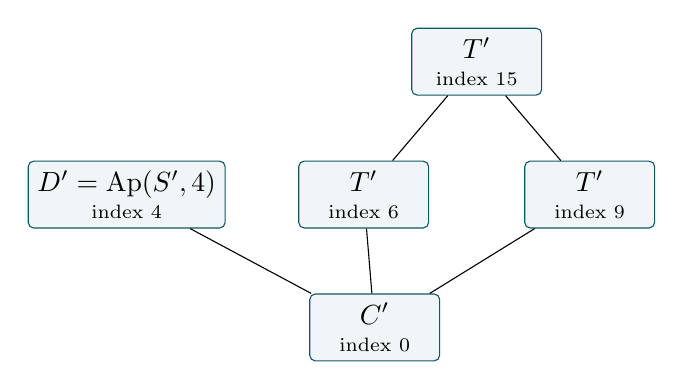
\begin{tikzpicture}[x=1.4cm,y=1.25cm,
  box/.style={draw=teal,rounded corners=2pt,fill=pale,
     minimum width=1.65cm,minimum height=0.68cm,align=center},
  every edge/.style={draw=ink,line width=0.6pt}]
\node[box] (base) at (0,0) {$C'$\\[-2pt]\scriptsize index 0};
\node[box] (d) at (-2.25,1.35) {$D'=\Ap(S',4)$\\[-2pt]\scriptsize index 4};
\node[box] (p) at (-0.1,1.35) {$T'$\\[-2pt]\scriptsize index 6};
\node[box] (q) at (1.95,1.35) {$T'$\\[-2pt]\scriptsize index 9};
\node[box] (r) at (0.925,2.7) {$T'$\\[-2pt]\scriptsize index 15};
\draw (base)--(d);\draw (base)--(p);\draw (base)--(q);
\draw (p)--(r);\draw (q)--(r);
\end{tikzpicture}
\caption{The exact residual block order for $\langle4,6,9\rangle$. Each
edge means that every element of the lower block lies below every element
of the upper block. The poisoned point is removed only from the block at
index 0. Compare \cref{fig:blocks}, the same diagram with the indices
$0,4,5,6,11$ of $\langle4,5,6\rangle$.}
\label{fig:blocks469}
\end{figure}

\begin{proof}[Proof of \cref{thm:second}]
Part (i). For $\sigma=0$ the board is $\{0\}$, which has no legal Chomp
move, so it is $\Pout$. For $\sigma=1$ it is \cref{lem:base469}.

Part (ii). \Cref{lem:gap469} below proves that every positive option of
$T'$ has value at least 3. The move at 0 has value 0, and the move at 4
has value 3 by \cref{eq:diamond469-value}. Hence
\[
 \opt(T')\cap\{0,1,2,3\}=\{0,3\},
\]
which with $\sg(C')=0$ is exactly \cref{eq:spectral-hypothesis}. All
option values of $T'$ are finite, since every option is a finite poset.
\Cref{prop:mechanism} therefore applies with $a=4$, $p=6$, $q=9$,
$r=15$; alternatively \cref{prop:criterion} applies, since 4 is an atom.
Either way $\sg\bigl((T'+T'):T'\bigr)=3$ by \cref{lem:detector}, so the
game in parentheses in \cref{eq:residual469} has value
$3\nimadd3=0$, and $\sg(R')=\sg(C')=0$ by \cref{lem:colon}. Thus
$\omega4+4$ leaves a $\Pout$-position and wins.

Part (iii). Let $\sigma>2$. Every $\beta\in S'^{\sigma}\setminus S'^{2}$
has leading exponent at least 2, so $(\omega4+4)+\beta=\beta$ and
therefore $\beta-(\omega4+4)=\beta\in S'^{\sigma}$. The move deletes every
such $\beta$ and leaves exactly the residual game of the square.

For minimality, no positive \emph{finite} opening wins: such a move
deletes every ordinal with a positive higher coefficient and leaves
$\Ap(S',b)\setminus\{0\}$, which is $\Nout$ by \cref{lem:base469}. The
only remaining legal opening below $\omega4+4$ is $\omega4$. After it the
block at index 4 is absent, and the opponent answers $\omega15$, deleting
the top block and leaving $C':(T'+T')$, which is $\Pout$ because
$\sg(C')=0$ and $\sg(T'+T')=1\nimadd1=0$. There are no intermediate legal
coefficients 1, 2, or 3, since those are gaps of $S'$. Hence $\omega4+4$
is the least winning opening, and $\ch(\{4,6,9\})=2$.
\end{proof}

\subsection{The poisoned--unpoisoned dictionary}
\label{sec:dictionary}

Two conventions for the same boards are in circulation, and the files
shipped with this report use both. It is worth fixing the translation
once, because every number quoted in \cref{sec:certificate469} from the
ported certificate is a poisoned number.

Throughout this article, $\sg(Q)$ is the \emph{unpoisoned} normal-play
value: the board is played with all of its listed elements, including its
least element 0 when present. The certificates
\path{certificates/s456.json} and \path{certificates/s469.json} follow
this convention, with $K=2$ and the saturation symbol $\sat$ written as
the digit 3, so that their labels mean
\[
 0=\text{exactly }0,\quad 1=\text{exactly }1,\quad
 2=\text{exactly }2,\quad \sat=\text{at least }3 .
\]
The certificate \path{certificates/s469_poisoned.json}, ported from the
second source report, instead records the poisoned boards
$Q\setminus\{0\}$, with the legend
\[
 \boxed{\quad 0=\text{exactly }0,\qquad
 1=\text{exactly }1,\qquad 2=\text{at least }2.\quad}
\]
In particular a poisoned label 2 does \emph{not} assert an exact value
of 2. By \cref{cor:min-shift} the two conventions are related by
\begin{equation}\label{eq:dictionary}
 \sg(Q)=1+\sg\bigl(Q\setminus\{0\}\bigr)
\end{equation}
for every finite board $Q$ with least element 0. Writing
\[
 q_x(C)=\min\bigl(2,\;\sg(P(x,C)\setminus\{0\})\bigr)
\]
for the poisoned truncated entry beside the unpoisoned $v_x(C)$ of
\cref{sec:window}, the label correspondence is
\begin{equation}\label{eq:label-dictionary}
 q_x(C)=0\;\leftrightarrow\;v_x(C)=1,\qquad
 q_x(C)=1\;\leftrightarrow\;v_x(C)=2,\qquad
 q_x(C)=2\;\leftrightarrow\;v_x(C)=\sat .
\end{equation}
Every poisoned number quoted below is one less than its unpoisoned
counterpart, and the saturation symbols correspond.

One consequence is \emph{not} a shift, and must be stated separately. The
far spectrum \cref{eq:far} equals $\{0\}$ in the unpoisoned convention,
as recorded in \cref{eq:far-constant}, because the unpoisoned move at
$y=0$ leaves the empty game, of value 0. In the poisoned convention that
move does not exist, the far prefix contributes nothing below the cutoff,
and the corresponding set is \emph{empty}. The statements ``$B_x=\{0\}$''
and ``$B_{23}=\varnothing$'' are the same fact in the two conventions;
neither contradicts the other. The same care is needed for the counts
reported in \cref{sec:checks469}.

\subsection{The seventeen gap ideals, in two orders}
\label{sec:ideals469}

Give $\HH'$ the order induced by semigroup differences. Its cover
relations are
\begin{equation}\label{eq:covers469}
 1\prec5,\quad 1\prec7,\quad 3\prec7,\quad
 2\prec11,\quad 5\prec11,\quad 7\prec11,
\end{equation}
and its downsets number 17. Encode a downset $C\subseteq\HH'$ by
\[
 m(C)=\mathbf1_{1\in C}+2\cdot\mathbf1_{2\in C}+4\cdot\mathbf1_{3\in C}
      +8\cdot\mathbf1_{5\in C}+16\cdot\mathbf1_{7\in C}
      +32\cdot\mathbf1_{11\in C}.
\]
\Cref{tab:ideals469} lists all seventeen as explicit sets, together with
their masks.

\begin{table}[htbp]
\centering\small
\begin{tabular}{r l r r @{\hspace{2.2em}} r l r r}
\toprule
$i$ & $C_i$ & $m(C_i)$ & $j$ & $i$ & $C_i$ & $m(C_i)$ & $j$\\
\midrule
0 & $\varnothing$ & 0 & 0 & 9 & $\{1,2,5\}$ & 11 & 9\\
1 & $\{1\}$ & 1 & 1 & 10 & $\{1,3,5\}$ & 13 & 10\\
2 & $\{2\}$ & 2 & 2 & 11 & $\{1,3,7\}$ & 21 & 12\\
3 & $\{3\}$ & 4 & 4 & 12 & $\{1,2,3,5\}$ & 15 & 11\\
4 & $\{1,2\}$ & 3 & 3 & 13 & $\{1,2,3,7\}$ & 23 & 13\\
5 & $\{1,3\}$ & 5 & 5 & 14 & $\{1,3,5,7\}$ & 29 & 14\\
6 & $\{1,5\}$ & 9 & 8 & 15 & $\{1,2,3,5,7\}$ & 31 & 15\\
7 & $\{2,3\}$ & 6 & 6 & 16 & $\HH'=\{1,2,3,5,7,11\}$ & 63 & 16\\
8 & $\{1,2,3\}$ & 7 & 7 & & & &\\
\bottomrule
\end{tabular}
\caption{The seventeen admissible gap tails of $\langle4,6,9\rangle$.
The index $i$ sorts them by cardinality and then lexicographically, which
is the column order of \texttt{certificates/s469\_poisoned.json} and of
\cref{app:certificate469}. The index $j$ sorts them by ascending mask,
which is the column order of \texttt{certificates/s469.json} and of
\texttt{data/s469\_low\_rows.csv}.}
\label{tab:ideals469}
\end{table}

\paragraph{Reconciling the two column orders.}
The two shipped certificates for this semigroup order these seventeen
downsets \emph{differently}, and this is the one place where a careless
comparison produces a spurious contradiction. The file
\path{certificates/s469.json} lists ascending masks,
\begin{equation}\label{eq:masks469}
 0,1,2,3,4,5,6,7,9,11,13,15,21,23,29,31,63,
\end{equation}
while \path{certificates/s469_poisoned.json} and
\cref{app:certificate469} use increasing cardinality and then
lexicographic order. With $j$ and $i$ as in \cref{tab:ideals469}, the
dictionary is $i=\pi(j)$ for
\begin{equation}\label{eq:column-perm}
 \pi=(0,1,2,4,3,5,7,8,6,9,10,12,11,13,14,15,16).
\end{equation}
The permutation transposes exactly three pairs of columns, namely
$\{3\}\leftrightarrow\{1,2\}$, $\{1,5\}\leftrightarrow\{2,3\}$, and
$\{1,3,7\}\leftrightarrow\{1,2,3,5\}$, and fixes the other eleven. Under
\cref{eq:column-perm} together with the label dictionary
\cref{eq:label-dictionary}, the two certificates agree in every one of
their $253\cdot17=4301$ entries, and their untruncated companion tables
\path{data/s469_exact_finite_audit.csv} and
\path{data/s469_poisoned_boundary_values.csv} agree in all 4301 exact
values, the second being the first minus one throughout. The verifier
\path{code/verify_poisoned_certificate.py} asserts this agreement cell by
cell on every run. A reader who compares two rows without applying
\cref{eq:column-perm} and \cref{eq:label-dictionary} and finds a
discrepancy has found an artefact of the two orderings, not a
disagreement between the certificates.

\subsection{Initial values and the specialized recurrence}
\label{sec:initial469}

There are five positive semigroup elements below the conductor. Their
exact Ap\'ery values, in both conventions, are
\begin{equation}\label{eq:early469}
\begin{array}{c|rrrrr}
 t&4&6&8&9&10\\\hline
 \sg\bigl(\Ap(S',t)\setminus\{0\}\bigr)&2&4&3&6&5\\[1pt]
 \sg\bigl(\Ap(S',t)\bigr)&3&5&4&7&6
\end{array}
\end{equation}
The second row is the first plus one, by \cref{eq:dictionary}. The file
\path{data/s469_poisoned_apery_values.csv} carries both rows, for these
five parameters and for every $x$ up to 264; it is the only shipped
artefact presenting the two conventions side by side, and it is the
machine-readable form of \cref{sec:dictionary}. In particular no
exceptional parameter has unpoisoned value below 3.

The eleven initial rows $12\leq x\leq22$ are computed directly from the
finite boards $P(x,C)$, without the moving-boundary recurrence. The
largest integer appearing in those initial boards is 33.

Because every exceptional value already meets the cutoff, the poisoned
far-prefix set $B_{23}$ is \emph{empty}, which by \cref{sec:dictionary}
is the same statement as the unpoisoned $B_x=\{0\}$ of
\cref{eq:far-constant}. The recurrence \cref{eq:recurrence} therefore
specializes, in the poisoned convention, to
\begin{equation}\label{eq:special469}
 q_x(C)=\pmex\Bigl(
   \{q_{x-d}(\Delta_d(C)):1\leq d\leq11\}
   \cup\{q_x(C_c):c\in C\}\Bigr),
 \qquad x\geq23,
\end{equation}
where $\pmex A=\min(2,\mex A)$, and $\Delta_d$ and $C\mapsto C_c$ are the
maps of \cref{eq:delta,eq:cut}. The poisoned sources call these two maps
$T_d$ and $R_a$; they are the same maps.

This simplification is \emph{checked inductively}; it is not a prior
assumption of the conclusion. Every computed full-tail coordinate must
remain 2 throughout the initial segment and throughout the certified
cycle, and the verifier fails otherwise.

\subsection{The certificate and its closure}
\label{sec:certificate469}

Write the seventeen-entry poisoned row as the word
\[
 w_x=q_x(C_0)q_x(C_1)\cdots q_x(C_{16})\in\{0,1,2\}^{17},
\]
in the column order of \cref{tab:ideals469}; its final digit is the
full-tail label. The certificate consists of the 253 words
$w_{12},\ldots,w_{264}$ printed in \cref{app:certificate469}, and has
three closure properties:
\begin{equation}\label{eq:closure469}
\begin{aligned}
 &q_x(C_{16})=2 &&(12\leq x\leq264),\\
 &(w_{226},\ldots,w_{236})=(w_{254},\ldots,w_{264}),&&\\
 &w_x\ \text{satisfies \cref{eq:special469}} &&(23\leq x\leq264).
\end{aligned}
\end{equation}
The middle line compares exactly $11\times17=187$ labels. It says that
the complete boundary state before row 237 equals the complete boundary
state before row 265, that is,
\begin{equation}\label{eq:repeat469}
 \boxed{\mathscr S_{237}=\mathscr S_{265},}
\end{equation}
and the period is $265-237=28$.

\begin{lemma}[Certified spectral gap for $\langle4,6,9\rangle$]
\label{lem:gap469}
For every $t\in S'\setminus\{0\}$,
\begin{equation}\label{eq:gap469}
 \sg\bigl(\Ap(S',t)\setminus\{0\}\bigr)\geq2,
\end{equation}
equivalently $\sg(\Ap(S',t))\geq3$: every positive option of the
unpoisoned game $T'$ has Grundy value at least 3.
\end{lemma}
\begin{proof}
The finite recursion verifies \cref{eq:early469}, the eleven initial
rows, and \cref{eq:closure469}. Each initial full-tail label is 2, so
$B_{23}=\varnothing$; inductively the specialized recurrence
\cref{eq:special469} is the general recurrence \cref{eq:recurrence} and
preserves the empty prefix set through row 264. The two complete boundary
states then coincide, and \cref{thm:window} applies: determinism makes
every subsequent state repeat the same cycle, in which each full-tail
label is again 2. Hence $q_t(\HH')=2$ for every $t\geq12$, and since
$\Ap(S',t)=P(t,\HH')$ for $t>F'$ by \cref{lem:tails}, the poisoned
Ap\'ery board has value at least 2 for all such $t$. The five exceptional
parameters below 12 are covered by \cref{eq:early469}. The unpoisoned
reformulation is \cref{eq:dictionary}.
\end{proof}

The row sequence is periodic from row 226 onward with period 28. The
ported verifier additionally checks $w_{225}\neq w_{253}$, so 226 is the
\emph{earliest} onset for this particular period; no assertion is made
about the least possible period. The analogous onset for
$\langle4,5,6\rangle$, period 8 from row 36, is recorded but is not
certified minimal, since \path{code/verify.py} performs no such check.

\subsection{What was independently checked}
\label{sec:checks469}

Beyond the generator-based checker and the untruncated audit described in
\cref{sec:reproduce}, this semigroup is examined by a third
implementation, working in the poisoned convention.

That verifier rebuilds semigroup membership from the generators 4, 6, and
9 rather than from a gap list; enumerates the seventeen downsets by a
deliberately different route, \texttt{itertools.combinations} rather than
bit masks; and computes \emph{untruncated} integer Grundy values with bit
masks. It directly solves all $253\times17=4301$ boards represented in
the certificate, not merely the eleven initial rows; its cache then holds
4346 distinct finite \emph{poisoned} states. The largest board element
used anywhere in these checks is $264+11=275$. It verifies 233 literal
local residual-poset identities at $x=23$ and cross-checks them against
the certificate's stored transition index tables; it then \emph{replays}
the bounded recurrence from those stored indices alone, consulting no
exact high value and no semigroup arithmetic. It checks the 187-entry
repeated state, the onset inequality $w_{225}\neq w_{253}$, the diamond,
asserting that its option set is exactly $\{0,1,2\}$ and not merely that
its value is 3, the finite gadget of \cref{sec:gadget}, the column
dictionary \cref{eq:column-perm}, and the SHA-256 digest of the
certificate bytes.

\paragraph{Conventions attach to counts.}
All counts in the preceding paragraph are \emph{poisoned}-convention
counts and must be read as such. In particular the 4346 memoized states
there and the 4347 distinct finite positions reported by
\path{code/independent_check.py} in \cref{sec:reproduce} are not in
conflict: the first solver works on boards with 0 deleted, the second on
boards with 0 retained. The same applies to the counts 233, 187, 275,
and 33, and to the pair $403/4347$ in the table of
\cref{sec:reproduce}.

\paragraph{The regression suite.}
Six tests accompany the ported verifier, and they have no counterpart in
the first source report. Among them,
\texttt{test\_general\_boundary\_recurrence} validates the identities
behind \cref{thm:window} on eight numerical semigroups,
\[
 \langle2,3\rangle,\ \langle3,4\rangle,\ \langle3,5\rangle,\
 \langle3,4,5\rangle,\ \langle4,5,6,7\rangle,\ \langle4,6,9\rangle,\
 \langle5,6,7\rangle,\ \langle6,7,8,9\rangle,
\]
at the three cutoffs 1, 2, 3; that is evidence for the general theorem
rather than for one semigroup. \texttt{test\_capped\_mex\_identity}
machine-checks \cref{eq:exact-truncation} over all 256 subsets of
$\{0,\ldots,7\}$ and cutoffs 1 through 5, an identity asserted but never
machine-checked in the first source report.
\texttt{test\_corrupted\_label\_rejected} and
\texttt{test\_corrupted\_transition\_rejected} are negative controls,
proving that the verifier is able to fail.
\texttt{test\_regeneration} pins the generator's output against the
shipped JSON. The recorded run is
\path{data/s469_poisoned_tests.txt}.

\paragraph{Two generators, one of which searches.}
The certificate builder \path{code/build_certificates.py} intentionally
replays the documented candidate repeat indices; it is a reproducible
generator, not a search program. The ported
\path{code/make_poisoned_certificate.py} is a search: it walks forward
keeping a dictionary of complete boundary states, \emph{discovers} the
first repetition at $237=265$ rather than being told where it is, and
then derives the onset
$226=1+\max\{x:w_x\neq w_{x+28}\}$. It is therefore the shipped code that
underwrites the onset claim.

\paragraph{The trust boundary.}
The mathematical trust boundary consists of ordinary mathematical
reasoning plus finite exact integer computations under Python. No
floating-point arithmetic, random search, external solver, or conjectured
period is involved. No formal proof-assistant verification is claimed.
The several implementations are separate implementations of the same
finite calculation, not two independent human proofs; they reduce coding
risk without substituting for a proof-assistant kernel or for independent
human review.

\subsection{A purely finite analogue of the three-block architecture}
\label{sec:gadget}

\Cref{lem:detector} is an algebraic statement about option spectra. It
admits a purely finite confirmation on an explicit finite poset, which
the ported verifier performs and which is logically independent of the
semigroup calculation. This is a genuinely different confirmation of the
whole three-block architecture, and it is not a truncation of an infinite
board; nothing in the first source report's code does it.

Let $H$ be the disjoint union of two two-element chains, and let
$P=\mathbf1:H$ be a minimum placed below both chains, so that
$H=P\setminus\{0\}$. Then
\[
 \sg(H)=2\nimadd2=0,\qquad \sg(P)=1,\qquad \opt(P)=\{0,3,4\},
\]
so $P$ has exactly the low spectrum $\opt(P)\cap\{0,1,2,3\}=\{0,3\}$
demanded by \cref{eq:low-spectrum}. Forming $K=(P+P):P$ gives
\[
 \sg(K)=3,
\]
which is \cref{eq:V-three} realized on a fifteen-point poset instead of
on an infinite board. Finally, writing $D'$ for the literal four-point
incidence matrix of $\Ap(S',4)$ computed from the generators,
\begin{equation}\label{eq:gadget}
 \sg\bigl(H:(D'+K)\bigr)=0,
\end{equation}
which is \cref{eq:remaining-general} on a finite poset with the block
order of \cref{fig:blocks469}. The value 0 is recorded as
\texttt{finite\_analogue\_residual\_value} in
\path{data/s469_poisoned_verification.json}.

\subsection{Concrete replies after the winning move}
\label{sec:replies469}

\Cref{sec:strategy} gives a general three-phase invariant argument that
names no ordinal moves, and it applies here verbatim after replacing the
diamond labels 5, 6, 11 by 6, 9, 15. The catalogue below is a second and
deliberately concrete derivation of the same replies: it names the actual
ordinal moves, and it is retained because it exercises the block
decomposition \cref{eq:residual469} directly, whereas the invariant
argument establishes only that a suitable finite move exists. Both are
kept; neither supersedes the other.

Let Alice have opened at $(4,4)$. Bob now moves in one of the five blocks
of \cref{fig:blocks469}.

\paragraph{Bob moves in the bottom block, $a=0$.}
Every upper block disappears. The residual is a finite poisoned Ap\'ery
board, of value at least 2 by \cref{lem:gap469}. Alice computes an
ordinary finite-poset move to value 0 and thereafter restores value 0
after each reply.

\paragraph{Bob moves in the diamond block, $a=4$.}
Let $d\in\{0,1,2\}$ be the remaining unpoisoned Grundy value of that
block. Alice changes the three-block component $K'=(T'+T'):T'$ to the
same value $d$:
\begin{center}
\begin{tabular}{ccl}
\toprule
$d$ & Alice's move & New three-block value\\
\midrule
$0$ & $(15,0)$ & $\sg(T'+T')=0$\\
$1$ & $(6,0)$ & $\sg(T')=1$\\
$2$ & $(6,4)$ & $\sg(D'+T')=3\nimadd1=2$\\
\bottomrule
\end{tabular}
\end{center}
The two independent upper components then cancel.

\paragraph{Bob moves in a middle block, $a=6$ or $a=9$.}
The top block at index 15 disappears. If Bob chose inner 0, Alice plays
$(4,15)$, leaving the diamond branch at value 1, which cancels the
untouched middle block. Otherwise Bob has left a finite unpoisoned
Ap\'ery board of value $b\geq3$; Alice moves inside that same finite
block to leave value 2, which is possible because $2<b$. The three
remaining independent upper values are then 2, 1, and 3, whose
exclusive-or is 0.

\paragraph{Bob moves in the top block, $a=15$.}
If he chose inner 0, Alice removes the whole diamond by playing $(4,0)$,
and the two untouched middle blocks cancel. Otherwise the finite top
residual has unpoisoned value at least 3, and Alice moves there to leave
value 1; the excluded-ordinal formula \cref{lem:colon} restores the
three-block value to 3, which again cancels the diamond.

Every described reply leaves a position of value 0, and the finite moves
to a requested smaller nimber are obtained by the same exact finite-poset
recursion used in the verifiers. This response analysis is not a claim of
a uniform polynomial-time strategy for arbitrary later ordinal-game
positions; the existence of the winning strategy already follows from the
proved zero-value residual together with termination.

\subsection{What is established, and what is not}
\label{sec:scope}

The result settles the stated minimal-transition question negatively and
refutes winner stability: a numerical-semigroup generator set can have
transition exponent strictly larger than its first admissible exponent.
It does not contradict the positive result for losing semigroups of
maximal embedding dimension in \cite[Proposition 4.2]{RH26}. Both
examples here have multiplicity 4 and three minimal generators, rather
than four minimal generators.

The universal assertion actually established is a low-value exclusion,
\[
 \sg\bigl(\Ap(S,t)\setminus\{0\}\bigr)\notin\{0,1\}\qquad(t>0),
\]
for each of the two semigroups. The raw Grundy values are not claimed to
be periodic. In particular the label 2 in the last column of the ported
certificate does \emph{not} mean that every Ap\'ery board has value 2:
the early exact values $2,4,3,6,5$ of \cref{eq:early469} already show
otherwise. Nor is the exponent 2 obtained by testing finitely many
exponents. It is established by proving a losing position at exponent 1,
giving an explicit winning move at exponent 2, and proving that this same
move removes every additional higher-order element.

We do not claim that these are the smallest counterexamples under every
possible measure of semigroup size. The minimality proved here concerns
the \emph{winning ordinal move} and the exact transition for these two
specified semigroups. We have not classified all semigroups with
transition 2, established a larger transition, or proved that an
unrestricted ordinal-level winner problem is decidable. A negative answer
to the minimal-transition question does not itself imply undecidability.

\subsection{Questions left open}

A natural next classification problem is to determine which numerical
semigroups have first winning exponent 2 and which preserve a
second-player win at every ordinal exponent. \Cref{prop:criterion}
supplies a searchable sufficient condition, but it is not a
characterization.

A second question is whether the transition exponents of finite
natural-number generating sets are bounded by a small finite ordinal.
Nothing here establishes such a bound or constructs an exponent above 2.

On the finite-state side, one can ask for a conceptual, non-computational
proof of the specific excluded value that would replace the certificate,
or for invariants that \emph{compress} its 187-entry state. The present
proof needs no such compression: all entries and the transition law are
already finite and explicit. The finite-window theorem
\cref{thm:window} also suggests systematic searches for other small
option-spectrum patterns that trigger an ordinal winner change, and it
identifies a reusable approach, since membership of any fixed finite
nimber in the one-move spectrum is effectively decidable. These are
further questions, not assumptions in the present proof.

\section{Reproducibility and verification boundaries}\label{sec:reproduce}

The archive contains the article source and PDF, three JSON certificates,
CSV tables, a minimal verifier, a general verifier, an independent finite
audit, a poisoned-convention verifier with its generator, table exporter
and regression suite, and the recorded verification output. No external
Python package is required, and no network access is used. The scripts
are written for Python 3.9 or later, with the unpoisoned scripts
assuming 3.10 or later. The runs recorded in \path{verification.txt},
\path{verification_poisoned.txt} and \path{data/s469_poisoned_tests.txt}
used Python 3.14.4 on this merged package; the two source reports
recorded their original runs under Python 3.13.5.

\subsection{Commands}

From the archive root, the unpoisoned checks are
\begin{lstlisting}[language={},basicstyle=\small\ttfamily]
python code/minimal_verifier.py
python code/verify.py
python code/independent_check.py
\end{lstlisting}
The first program is the complete small recurrence check printed in
\cref{app:code}. The second recomputes the gap sets from the given
generators, constructs every admissible gap downset, verifies the seed
rows and each recurrence row, checks the exceptional parameters, and
compares the complete repeated states. The third does not import the
recurrence implementation: it builds principal upper sets from the
generators, encodes finite positions as bit masks, and computes
\emph{full} Grundy numbers by literal move enumeration. Both of the last
two scan the certificates directory for names matching the pattern
\texttt{s4}\textit{dd}\texttt{.json} only, so that the poisoned
certificate described below is not handed to a verifier expecting the
unpoisoned schema.

The poisoned-convention checks, which concern $\langle4,6,9\rangle$ only,
are
\begin{lstlisting}[language={},basicstyle=\small\ttfamily]
python code/verify_poisoned_certificate.py
python code/test_poisoned_certificate.py
\end{lstlisting}
and the two regeneration steps are
\begin{lstlisting}[language={},basicstyle=\small\ttfamily]
python code/build_certificates.py
python code/make_poisoned_certificate.py
python code/export_poisoned_tables.py
\end{lstlisting}
The targets \texttt{make verify}, \texttt{make test},
\texttt{make certificates} and \texttt{make pdf} wrap these.
\path{build.ps1} runs the verifiers, the test suite and the three
\LaTeX\ passes on Windows PowerShell, but not the regeneration step, so
\texttt{make certificates} has no PowerShell counterpart. That
PowerShell wrapper is supplied for convenience; it was not executed in
the Linux verification environment in which the original poisoned checks
were run.

\subsection{The three certificates}

Three certificate files are shipped, for two semigroups.
\begin{center}
\begin{tabular}{@{}p{0.34\textwidth}llp{0.2\textwidth}@{}}
\toprule
File & Semigroup & Convention & Column order\\
\midrule
\path{certificates/s456.json} & $\langle4,5,6\rangle$
  & unpoisoned, $\sat=3$ & ascending masks\\
\path{certificates/s469.json} & $\langle4,6,9\rangle$
  & unpoisoned, $\sat=3$ & ascending masks\\
\path{certificates/s469_poisoned.json} & $\langle4,6,9\rangle$
  & poisoned, $2=$ ``at least 2'' & cardinality, then lex\\
\bottomrule
\end{tabular}
\end{center}
The last two describe the \emph{same} 253 rows over the same seventeen
gap ideals; \cref{sec:ideals469} gives the exact dictionary, and
\path{code/verify_poisoned_certificate.py} checks it. Both are kept: the
poisoned file is the only one carrying the transition index tables
\texttt{transition\_recent\_indices} and
\texttt{transition\_tail\_indices}, the fields \texttt{label\_meaning},
\texttt{convention}, \texttt{conductor}, \texttt{frobenius},
\texttt{cutoff}, \texttt{period\_start} and
\texttt{early\_apery\_values}, and the published digest.

\subsection{The digest}

The poisoned certificate has
\begin{center}
\texttt{\footnotesize SHA-256 =
f408697a728c12efd4cca15b73d055b3c747a17e5b06a5897969973ceb1697dc,}
\end{center}
recorded in \path{data/s469_poisoned_verification.json},
\path{verification_poisoned.txt} and the README. This digest stays valid
only while the file is preserved byte for byte; any reformatting,
re-indentation, key reordering or change of line endings would silently
invalidate it. The generator therefore writes the file with explicit
\texttt{"\textbackslash n"} line endings, so that regeneration on any
platform reproduces the same bytes, and the verifier recomputes and
prints the digest on every run. Repository-wide \path{SHA256SUMS.txt}
manifests are no longer distributed, so this is the only per-file
integrity claim in the archive. Recompiling the document may change the
PDF's byte hash, because of timestamps and TeX versions; the JSON
certificates are deterministic.

\subsection{What the executed checks reported}

\begin{center}
\begin{tabular}{llrrr}
\toprule
Semigroup & Convention & Certificate entries & Direct finite states
 & State repetition\\
\midrule
$\langle4,5,6\rangle$ & unpoisoned & 387 & 403 & $43=51$\\
$\langle4,6,9\rangle$ & unpoisoned & 4301 & 4347 & $237=265$\\
$\langle4,6,9\rangle$ & poisoned & 4301 & 4346 & $237=265$\\
\bottomrule
\end{tabular}
\end{center}
``Direct finite states'' counts distinct positions visited by the
corresponding independent recursive evaluator, not all possible
infinite-game states. The two counts for $\langle4,6,9\rangle$ differ by
exactly the convention, as explained in \cref{sec:checks469}: 4347
unpoisoned boards against 4346 poisoned ones. The files
\path{verification.txt} and \path{verification_poisoned.txt} record the
actual outputs, and \path{data/s469_poisoned_tests.txt} records the
regression run, with all six tests passing.

\subsection{Why a finite certificate proves an infinite assertion}

There are three separate verification obligations. The code checks the
finite values and the repeated states. The proof of \cref{thm:window}
explains why a repeated state covers all larger parameters. Finally, the
order decomposition and the game algebra, or equivalently the response
procedures of \cref{sec:strategy,sec:replies469}, connect the spectral
fact to the ordinal opening. A direct finite audit alone would not
replace either of the latter two mathematical arguments.

It is worth stating the negative version explicitly. No assertion about
an infinite board is inferred merely from a large finite truncation. The
complete state is an eleven-row window for $\langle4,6,9\rangle$ and a
seven-row window for $\langle4,5,6\rangle$, together with the accumulated
far spectrum; once that window repeats, the same deterministic operation
repeats forever. The exact, unbounded Grundy sequence is not claimed to
be eventually periodic; only each fixed bounded profile is, as
\cref{rem:bounded} records.

To rebuild the document, use \texttt{make pdf}, which runs pdf\LaTeX{}
three times to settle the table of contents and cross-references, or run
\path{build.ps1}. The numerical certificates are independent of the
document-build process.

\appendix
\clearpage
\section{The complete certificate for
 \texorpdfstring{$\langle4,5,6\rangle$}{<4,5,6>}}\label{app:table}

Column labels are the shape masks in \cref{eq:shape-order};
$\sat$ denotes a Grundy value at least 3, so these are
\emph{unpoisoned} labels. The first seven rows are
seeds. The shaded rows 36--42 repeat at 44--50; the row at 43 is
computed from the first repeated window. Every last-column entry
is saturated. The same data are in \path{certificates/s456.json}.

\begin{center}
{\small\renewcommand{\arraystretch}{0.94}
\begin{tabular}{r*{9}{c}}
\toprule
$x$ & $0$ & $1$ & $2$ & $3$ & $4$ & $5$ & $6$ & $7$ & $15$\\
\midrule
8 & $2$ & $\sat$ & $\sat$ & $2$ & $\sat$ & $2$ & $2$ & $\sat$ & $\sat$\\
9 & $\sat$ & $2$ & $1$ & $\sat$ & $\sat$ & $\sat$ & $2$ & $1$ & $\sat$\\
10 & $2$ & $\sat$ & $\sat$ & $\sat$ & $\sat$ & $\sat$ & $2$ & $1$ & $\sat$\\
11 & $\sat$ & $\sat$ & $\sat$ & $\sat$ & $\sat$ & $\sat$ & $\sat$ & $\sat$ & $\sat$\\
12 & $2$ & $1$ & $\sat$ & $2$ & $\sat$ & $2$ & $2$ & $1$ & $\sat$\\
13 & $\sat$ & $2$ & $2$ & $\sat$ & $\sat$ & $\sat$ & $\sat$ & $\sat$ & $\sat$\\
14 & $2$ & $\sat$ & $\sat$ & $\sat$ & $\sat$ & $\sat$ & $2$ & $1$ & $\sat$\\
\midrule
15 & $\sat$ & $\sat$ & $\sat$ & $1$ & $\sat$ & $\sat$ & $\sat$ & $\sat$ & $\sat$\\
16 & $2$ & $\sat$ & $\sat$ & $2$ & $\sat$ & $2$ & $2$ & $\sat$ & $\sat$\\
17 & $\sat$ & $2$ & $2$ & $\sat$ & $\sat$ & $\sat$ & $\sat$ & $\sat$ & $\sat$\\
18 & $2$ & $\sat$ & $\sat$ & $\sat$ & $\sat$ & $\sat$ & $2$ & $\sat$ & $\sat$\\
19 & $\sat$ & $\sat$ & $\sat$ & $\sat$ & $\sat$ & $\sat$ & $\sat$ & $\sat$ & $\sat$\\
20 & $2$ & $1$ & $\sat$ & $2$ & $\sat$ & $2$ & $2$ & $1$ & $\sat$\\
21 & $\sat$ & $2$ & $2$ & $\sat$ & $\sat$ & $\sat$ & $\sat$ & $\sat$ & $\sat$\\
22 & $2$ & $1$ & $\sat$ & $\sat$ & $\sat$ & $\sat$ & $2$ & $1$ & $\sat$\\
23 & $1$ & $\sat$ & $\sat$ & $1$ & $\sat$ & $1$ & $1$ & $\sat$ & $\sat$\\
24 & $2$ & $\sat$ & $\sat$ & $2$ & $\sat$ & $1$ & $2$ & $\sat$ & $\sat$\\
25 & $\sat$ & $2$ & $1$ & $\sat$ & $\sat$ & $\sat$ & $2$ & $\sat$ & $\sat$\\
26 & $2$ & $\sat$ & $\sat$ & $\sat$ & $\sat$ & $2$ & $2$ & $\sat$ & $\sat$\\
27 & $\sat$ & $\sat$ & $\sat$ & $\sat$ & $\sat$ & $\sat$ & $\sat$ & $\sat$ & $\sat$\\
28 & $2$ & $1$ & $\sat$ & $\sat$ & $\sat$ & $\sat$ & $2$ & $1$ & $\sat$\\
29 & $\sat$ & $2$ & $2$ & $\sat$ & $\sat$ & $\sat$ & $\sat$ & $\sat$ & $\sat$\\
30 & $2$ & $1$ & $\sat$ & $2$ & $\sat$ & $\sat$ & $2$ & $1$ & $\sat$\\
31 & $1$ & $2$ & $\sat$ & $1$ & $\sat$ & $1$ & $1$ & $\sat$ & $\sat$\\
32 & $2$ & $\sat$ & $\sat$ & $2$ & $\sat$ & $1$ & $2$ & $\sat$ & $\sat$\\
33 & $\sat$ & $\sat$ & $1$ & $\sat$ & $\sat$ & $\sat$ & $\sat$ & $\sat$ & $\sat$\\
34 & $2$ & $\sat$ & $\sat$ & $2$ & $\sat$ & $2$ & $2$ & $\sat$ & $\sat$\\
35 & $\sat$ & $\sat$ & $\sat$ & $\sat$ & $\sat$ & $\sat$ & $\sat$ & $\sat$ & $\sat$\\
\midrule
\rowcolor{pale}
36 & $2$ & $1$ & $\sat$ & $\sat$ & $\sat$ & $\sat$ & $2$ & $1$ & $\sat$\\
\rowcolor{pale}
37 & $\sat$ & $\sat$ & $\sat$ & $\sat$ & $\sat$ & $\sat$ & $\sat$ & $\sat$ & $\sat$\\
\rowcolor{pale}
38 & $2$ & $1$ & $\sat$ & $2$ & $\sat$ & $2$ & $2$ & $1$ & $\sat$\\
\rowcolor{pale}
39 & $1$ & $2$ & $2$ & $1$ & $\sat$ & $1$ & $1$ & $\sat$ & $\sat$\\
\rowcolor{pale}
40 & $2$ & $\sat$ & $\sat$ & $\sat$ & $\sat$ & $1$ & $2$ & $\sat$ & $\sat$\\
\rowcolor{pale}
41 & $\sat$ & $\sat$ & $1$ & $\sat$ & $\sat$ & $\sat$ & $\sat$ & $\sat$ & $\sat$\\
\rowcolor{pale}
42 & $2$ & $\sat$ & $\sat$ & $2$ & $\sat$ & $2$ & $2$ & $\sat$ & $\sat$\\
\midrule
43 & $\sat$ & $2$ & $2$ & $\sat$ & $\sat$ & $\sat$ & $\sat$ & $\sat$ & $\sat$\\
\midrule
\rowcolor{pale}
44 & $2$ & $1$ & $\sat$ & $\sat$ & $\sat$ & $\sat$ & $2$ & $1$ & $\sat$\\
\rowcolor{pale}
45 & $\sat$ & $\sat$ & $\sat$ & $\sat$ & $\sat$ & $\sat$ & $\sat$ & $\sat$ & $\sat$\\
\rowcolor{pale}
46 & $2$ & $1$ & $\sat$ & $2$ & $\sat$ & $2$ & $2$ & $1$ & $\sat$\\
\rowcolor{pale}
47 & $1$ & $2$ & $2$ & $1$ & $\sat$ & $1$ & $1$ & $\sat$ & $\sat$\\
\rowcolor{pale}
48 & $2$ & $\sat$ & $\sat$ & $\sat$ & $\sat$ & $1$ & $2$ & $\sat$ & $\sat$\\
\rowcolor{pale}
49 & $\sat$ & $\sat$ & $1$ & $\sat$ & $\sat$ & $\sat$ & $\sat$ & $\sat$ & $\sat$\\
\rowcolor{pale}
50 & $2$ & $\sat$ & $\sat$ & $2$ & $\sat$ & $2$ & $2$ & $\sat$ & $\sat$\\
\bottomrule
\end{tabular}}

\end{center}

\clearpage
\section{The complete certificate for
 \texorpdfstring{$\langle4,6,9\rangle$}{<4,6,9>}}\label{app:certificate469}

Each word has seventeen digits, in the column order $i$ of
\cref{tab:ideals469}, which is \emph{not} the mask order used in
\cref{app:table}; see \cref{eq:column-perm}. These are \emph{poisoned}
labels, so a digit 2 means ``Grundy value at least 2'' for the board with
0 deleted, equivalently at least 3 for the unpoisoned board; see
\cref{eq:label-dictionary}. The final digit of each word is the full-tail
label. The first eleven words, $w_{12},\ldots,w_{22}$, are the initial
conditions; every subsequent word follows from \cref{eq:special469}. The
blocks $226$--$236$ and $254$--$264$ are identical, which is
\cref{eq:repeat469}. The table is printed in three independent
index--word columns, read downward within each column. The same data are
in \path{certificates/s469_poisoned.json}, and the unpoisoned form of the
same rows, in mask order, is in \path{certificates/s469.json}.

\begingroup
\footnotesize
\setlength{\tabcolsep}{5pt}
\renewcommand{\arraystretch}{1.03}
\begin{longtable}{r l @{\hspace{7pt}} r l @{\hspace{7pt}} r l}
\caption{All 253 certified bounded-Grundy row vectors.}\label{tab:certificate}\\
\toprule
$x$ & $w_x$ & $x$ & $w_x$ & $x$ & $w_x$\\
\midrule
\endfirsthead
\toprule
$x$ & $w_x$ & $x$ & $w_x$ & $x$ & $w_x$\\
\midrule
\endhead
\midrule
\multicolumn{6}{r}{\small Continued on the next page}\\
\endfoot
\bottomrule
\endlastfoot
12 & \texttt{12222122222211102} & 97 & \texttt{10222122220222122} & 182 & \texttt{21212002212220222}\\
13 & \texttt{21022222021222202} & 98 & \texttt{22222001221120222} & 183 & \texttt{22221222222222212}\\
14 & \texttt{22222112222221202} & 99 & \texttt{22222222222222222} & 184 & \texttt{02222021212200022}\\
15 & \texttt{22222222222222222} & 100 & \texttt{02222022222200022} & 185 & \texttt{10222222220222122}\\
16 & \texttt{12222122222211122} & 101 & \texttt{20222222220222222} & 186 & \texttt{22222001222220222}\\
17 & \texttt{21222222221222222} & 102 & \texttt{12221001221120222} & 187 & \texttt{22222222222222222}\\
18 & \texttt{22222112222221202} & 103 & \texttt{21122222221222222} & 188 & \texttt{02222022122200012}\\
19 & \texttt{22222222222222222} & 104 & \texttt{02112022222200012} & 189 & \texttt{20222222220222222}\\
20 & \texttt{12222122220211102} & 105 & \texttt{20221222220212222} & 190 & \texttt{22222002222220222}\\
21 & \texttt{21222222221222222} & 106 & \texttt{12221001221120222} & 191 & \texttt{22222222222222222}\\
22 & \texttt{22222112222221202} & 107 & \texttt{21122222221222222} & 192 & \texttt{02221021222200022}\\
23 & \texttt{22222222222222222} & 108 & \texttt{02122022222200012} & 193 & \texttt{20222222220222222}\\
24 & \texttt{12222122222211122} & 109 & \texttt{20222221220222222} & 194 & \texttt{22222002222220222}\\
25 & \texttt{21222222221222222} & 110 & \texttt{12222001221220222} & 195 & \texttt{22122222122222212}\\
26 & \texttt{22202112222221202} & 111 & \texttt{21222222221222222} & 196 & \texttt{02212022122200012}\\
27 & \texttt{22220222222202222} & 112 & \texttt{02222022222200022} & 197 & \texttt{20221222220212222}\\
28 & \texttt{12222122220211102} & 113 & \texttt{20221221220222222} & 198 & \texttt{21222002111220222}\\
29 & \texttt{21222222221222222} & 114 & \texttt{22222002221220222} & 199 & \texttt{22222222222222222}\\
30 & \texttt{22222112222221202} & 115 & \texttt{22222222222222222} & 200 & \texttt{02221021222200022}\\
31 & \texttt{22222222222222222} & 116 & \texttt{02222021222200022} & 201 & \texttt{20222222220222222}\\
32 & \texttt{12222102222211102} & 117 & \texttt{20122222220222222} & 202 & \texttt{22212002212220222}\\
33 & \texttt{21222222221222222} & 118 & \texttt{22221002222210222} & 203 & \texttt{22222222122222212}\\
34 & \texttt{22222112222221222} & 119 & \texttt{22222222222222222} & 204 & \texttt{02222022222200022}\\
35 & \texttt{22022222022222202} & 120 & \texttt{01112022122200012} & 205 & \texttt{20222222220222222}\\
36 & \texttt{12222122222211102} & 121 & \texttt{20221222220212222} & 206 & \texttt{22222002222220222}\\
37 & \texttt{21222222221222222} & 122 & \texttt{22212002122220212} & 207 & \texttt{22222222222222222}\\
38 & \texttt{22222112220221202} & 123 & \texttt{12221122222212122} & 208 & \texttt{02122022122200012}\\
39 & \texttt{22222222222222222} & 124 & \texttt{02221022222200012} & 209 & \texttt{10222221210222222}\\
40 & \texttt{12222122222211102} & 125 & \texttt{20222222220222222} & 210 & \texttt{21122002221220222}\\
41 & \texttt{21222222221222222} & 126 & \texttt{22222001212220222} & 211 & \texttt{22212222122222212}\\
42 & \texttt{22222102212221202} & 127 & \texttt{22222222222222222} & 212 & \texttt{02222022222200022}\\
43 & \texttt{22222222222222222} & 128 & \texttt{02222022222200022} & 213 & \texttt{20221222220212222}\\
44 & \texttt{12222122222211102} & 129 & \texttt{20222222220222222} & 214 & \texttt{22222002222220222}\\
45 & \texttt{21220222221202222} & 130 & \texttt{22222002222220222} & 215 & \texttt{21212222212221222}\\
46 & \texttt{22222112222221222} & 131 & \texttt{22222222222222222} & 216 & \texttt{02222022122200012}\\
47 & \texttt{22222222222222222} & 132 & \texttt{02222022121100012} & 217 & \texttt{20222221220222222}\\
48 & \texttt{12222122222211102} & 133 & \texttt{20222222220222222} & 218 & \texttt{21222002221220222}\\
49 & \texttt{21222222221222222} & 134 & \texttt{21222002221220212} & 219 & \texttt{22222222222222222}\\
50 & \texttt{22222112220221202} & 135 & \texttt{22222222222222222} & 220 & \texttt{02222022222200022}\\
51 & \texttt{22222222222222222} & 136 & \texttt{01212022212200022} & 221 & \texttt{20221222220212222}\\
52 & \texttt{12222122222211122} & 137 & \texttt{20221222220212222} & 222 & \texttt{22222002222220222}\\
53 & \texttt{21222222221222222} & 138 & \texttt{22212002212220222} & 223 & \texttt{12221121222222122}\\
54 & \texttt{22222102212221202} & 139 & \texttt{12222122222222122} & 224 & \texttt{02222021222200022}\\
55 & \texttt{22222222222222222} & 140 & \texttt{02222021222200022} & 225 & \texttt{20122222220222222}\\
56 & \texttt{12222122220211102} & 141 & \texttt{20222222220222222} & 226 & \texttt{22221002222210222}\\
57 & \texttt{21022222021222202} & 142 & \texttt{22222002121120212} & 227 & \texttt{22222222222222222}\\
58 & \texttt{22222112222221202} & 143 & \texttt{22222222222222222} & 228 & \texttt{02222022222200022}\\
59 & \texttt{22222222222222222} & 144 & \texttt{02222022222200022} & 229 & \texttt{20122222120222212}\\
60 & \texttt{12222102222211102} & 145 & \texttt{20222222220222222} & 230 & \texttt{12222001222220222}\\
61 & \texttt{21222222221222222} & 146 & \texttt{21212002212220222} & 231 & \texttt{21122222221222222}\\
62 & \texttt{22222112222221202} & 147 & \texttt{22221222222212222} & 232 & \texttt{02221022222200012}\\
63 & \texttt{22022222222202222} & 148 & \texttt{02212012222200012} & 233 & \texttt{20222222220222222}\\
64 & \texttt{12222122222211102} & 149 & \texttt{10222122220222122} & 234 & \texttt{22122002122220212}\\
65 & \texttt{21222222221222222} & 150 & \texttt{22222002122220212} & 235 & \texttt{22122222222212222}\\
66 & \texttt{22222112222221202} & 151 & \texttt{22122222122222222} & 236 & \texttt{02112022222200012}\\
67 & \texttt{22222222222222222} & 152 & \texttt{02221022222200012} & 237 & \texttt{20212222120222212}\\
68 & \texttt{12222122222211122} & 153 & \texttt{20222222220222222} & 238 & \texttt{22222002212220222}\\
69 & \texttt{21222222221222222} & 154 & \texttt{22222002222220222} & 239 & \texttt{22222222122222212}\\
70 & \texttt{22222112222221222} & 155 & \texttt{22221221222222222} & 240 & \texttt{02222022222200022}\\
71 & \texttt{22222222222222222} & 156 & \texttt{02222021222200022} & 241 & \texttt{20222222220222222}\\
72 & \texttt{12222122220211102} & 157 & \texttt{20122222220222222} & 242 & \texttt{22222002222220222}\\
73 & \texttt{21222222221222222} & 158 & \texttt{22222002222210222} & 243 & \texttt{22222222222222222}\\
74 & \texttt{22222112220221202} & 159 & \texttt{22222222222222222} & 244 & \texttt{02222022122200012}\\
75 & \texttt{22222222222222222} & 160 & \texttt{02222022121100012} & 245 & \texttt{20222222220222222}\\
76 & \texttt{10222122202211022} & 161 & \texttt{20222222220222222} & 246 & \texttt{22221002222210222}\\
77 & \texttt{21222222221222222} & 162 & \texttt{22222002221220212} & 247 & \texttt{22222222222222222}\\
78 & \texttt{22202102212221122} & 163 & \texttt{22222222222222222} & 248 & \texttt{02222022222200022}\\
79 & \texttt{02222022222222022} & 164 & \texttt{01222022212200022} & 249 & \texttt{20221222220212222}\\
80 & \texttt{12222122220221202} & 165 & \texttt{20222222220222222} & 250 & \texttt{22222002222220222}\\
81 & \texttt{21022222021222222} & 166 & \texttt{22212002212220222} & 251 & \texttt{12221121222222122}\\
82 & \texttt{22222112222201222} & 167 & \texttt{12222122222222122} & 252 & \texttt{02222022222200022}\\
83 & \texttt{22222222222222222} & 168 & \texttt{02222021221200022} & 253 & \texttt{20222222220222222}\\
84 & \texttt{10222122202210022} & 169 & \texttt{20222222220222222} & 254 & \texttt{22221002222210222}\\
85 & \texttt{21222222221222222} & 170 & \texttt{22222002221220212} & 255 & \texttt{22222222222222222}\\
86 & \texttt{12222120212221122} & 171 & \texttt{22222222222222222} & 256 & \texttt{02222022222200022}\\
87 & \texttt{01222022221222022} & 172 & \texttt{01222022211200022} & 257 & \texttt{20122222120222212}\\
88 & \texttt{12222021222100022} & 173 & \texttt{20222222220222222} & 258 & \texttt{12222001222220222}\\
89 & \texttt{21222222221222222} & 174 & \texttt{21212002212220222} & 259 & \texttt{21122222221222222}\\
90 & \texttt{21222002121220212} & 175 & \texttt{12222122222222122} & 260 & \texttt{02221022222200012}\\
91 & \texttt{22222222222222222} & 176 & \texttt{02222011222200022} & 261 & \texttt{20222222220222222}\\
92 & \texttt{01212022212200022} & 177 & \texttt{10222122220222222} & 262 & \texttt{22122002122220212}\\
93 & \texttt{10221122220212122} & 178 & \texttt{22222002121120212} & 263 & \texttt{22122222222212222}\\
94 & \texttt{21222001212220122} & 179 & \texttt{22122222122222212} & 264 & \texttt{02112022222200012}\\
95 & \texttt{22222222222222222} & 180 & \texttt{02221022222200012} &  & \\
96 & \texttt{02222021212200022} & 181 & \texttt{20222222220222222} &  & \\
\end{longtable}
\endgroup


\clearpage
\section{A self-contained verifier for the main spectral lemma}
\label{app:code}

This program computes the seeds directly, evolves the seven-row state,
and checks its repetition. Here 3 is a saturation marker. Run it
without Python's \texttt{-O}, which disables assertions. The longer
verifier uses explicit checks and derives the gap set from the generators.

\lstinputlisting[basicstyle=\fontsize{8.3}{9.2}\selectfont\ttfamily]{code/minimal_verifier.py}

\clearpage
\section{A compact statement of the checking algorithm}
\label{app:algorithm}

\Cref{app:code} prints a complete program for the smaller semigroup. For
$\langle4,6,9\rangle$ the analogous listing would be longer, so we state
only the mathematical core of the recurrence check. Here \texttt{tails}
is the list of gap ideals in the order of \cref{tab:ideals469},
\texttt{index} maps each ideal to its column, \texttt{rows} contains the
already checked words, and \texttt{member(n)} tests $n\geq0$ and
$n\notin\{1,2,3,5,7,11\}$. The values are poisoned labels.

\begin{lstlisting}
def next_row(x, rows, tails, index):
    result = []
    for C in tails:                # increasing cardinality
        options = set()
        for d in range(1, 12):
            T = frozenset(g for g in gaps
                          if g < d or g - d in C)
            options.add(rows[x - d][index[T]])
        for a in C:
            R = frozenset(g for g in C if not member(g - a))
            options.add(result[index[R]])
        value = 0
        while value in options:
            value += 1
        result.append(min(2, value))
    return tuple(result)
\end{lstlisting}

The actual verifier reconstructs the membership test from the generators
4, 6 and 9 rather than from the printed gap list. The omitted far-prefix
contribution is justified by checking that the initial exceptional
Ap\'ery values and all full-tail coordinates are at least 2, as in
\cref{sec:initial469}. The complete state is then an eleven-row window;
once that window repeats, the same deterministic operation repeats
forever.

For the finite seed calculation, and for the independent exhaustive
check, the only game-theoretic recursion needed is the literal
set-deletion form of \cref{eq:sg}:
\begin{equation}\label{eq:literal-mex}
 \sg(A)=\mex\bigl\{\sg\bigl(\{z\in A:z-y\notin S\}\bigr):y\in A\bigr\},
 \qquad \sg(\varnothing)=0.
\end{equation}
All sets $A$ here are finite sets of nonnegative integers. Each recursive
argument is a proper subset of $A$, so the calculation terminates by
induction on $|A|$. The bit-mask verifiers implement exactly this
recurrence, with exact, unrestricted nonnegative-integer values.

\clearpage
\begin{thebibliography}{9}
\addcontentsline{toc}{section}{References}

\bibitem{RH26}
Fabi\'an Rivero Herrera,
\emph{Hanf numbers for poset games},
arXiv:2504.07317v3, January 5, 2026.
Target: Question 4.6, credited in that revision to Ignacio
Garc\'ia-Marco; generated ordinal posets in Section 2; see also
Example 3.2 for winner changes among arbitrary finite pointed posets,
and Proposition 4.2 for maximal embedding dimension.
\url{https://arxiv.org/abs/2504.07317v3}.

\bibitem{RH25}
Fabi\'an Rivero Herrera,
\emph{A poset game in submonoids of additively indecomposable ordinals},
arXiv:2504.07317v1, April 9, 2025.
Earlier formulation: Conjecture 4.1, the winner-stability assertion
refuted here.
\url{https://arxiv.org/abs/2504.07317v1}.

\bibitem{GMK18}
Ignacio Garc\'ia-Marco and Kolja Knauer,
\emph{Chomp on numerical semigroups},
Algebraic Combinatorics \textbf{1} (2018), no.~3, 371--394.
\href{https://doi.org/10.5802/alco.16}{doi:10.5802/alco.16}.
Theorem 2.4 supplies the symmetric-semigroup outcome argument;
Section 6 develops finite-gap locality, which \cref{lem:tails} refines.
The study of this game originates here.
Preprint: \url{https://arxiv.org/abs/1705.11034}.
\url{https://alco.centre-mersenne.org/articles/10.5802/alco.16/}.

\bibitem{GT21}
Mi\v{s}o Gavrilovi\'c and Alexander Thumm,
\emph{The Ordered Join of Impartial Games},
arXiv:2104.13131v2, May 18, 2021.
Section 2 treats Grundy sets and the ordinal-sum formula; see especially
Theorem 2.6, on which \cref{cor:min-shift} leans, and Section 4 for the
ordered-join substitution theory of \cref{rem:substitution}.
\url{https://arxiv.org/abs/2104.13131v2}.

\end{thebibliography}
\end{document}
